\begin{figure*}[ht]
\subfigure[]{
 \resizebox{0.325\textwidth}{!}{
\schemestart
E\arrow(aa--bb){<=>[$k^{\prime}_R$][$k_R$]}[,,,red] $ER^*$
\arrow(--cc){<=>[$m'$][$m$]}[-90,,,red]$ER$
\arrow(@cc--@aa){<=>[$l^{\prime}_R$][$l_R$]}[,,,red]
\arrow(@aa--dd){<=>[$k_W$][$k^{\prime}_W$]}[180,,,red] $EW^*$
\arrow(--ee){<=>[${m'}$][${m}$]}[-90,,,red] $EW$
\arrow(@ee--@aa){<=>[$l_W$][$l^{\prime}_W$]}[,,,red]
\schemestop

}} 
\subfigure[]{
\resizebox{0.4\textwidth}{!}{
% This file was created by matlab2tikz.
%
%The latest updates can be retrieved from
%  http://www.mathworks.com/matlabcentral/fileexchange/22022-matlab2tikz-matlab2tikz
%where you can also make suggestions and rate matlab2tikz.
%
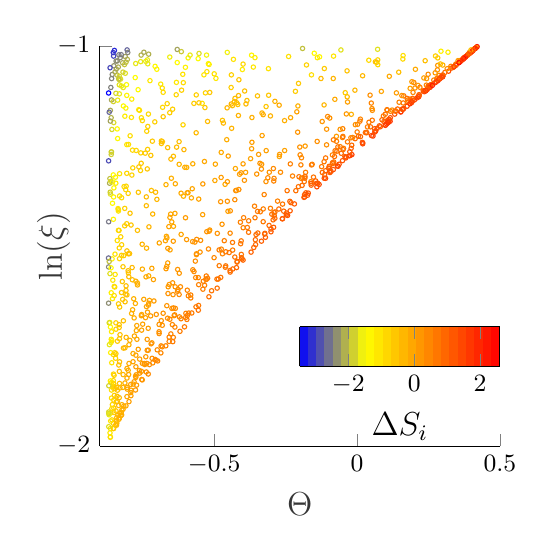
\begin{tikzpicture}[scale=1]

\begin{axis}[%
width=2in,
height=2in,
at={(0in,0in)},
scale only axis,
xmin=-0.9,
xmax=0.5,
xtick={-0.5,0,0.5},
xlabel style={font=\large\bfseries\color{white!21!black}},
xlabel={$\Theta$},
xticklabel style = {font=\small},
ymin=-2,
ymax=-1,
ytick={-2,-1},
ylabel style={font=\large\bfseries\color{white!21!black}, at={(axis description cs:-0.05,0.5)}},
ylabel={$\ln(\xi)$},
yticklabel style = {font=\small},
axis background/.style={fill=white},
axis x line*=bottom,
axis y line*=left,
legend style={legend cell align=left, align=left, draw=white!15!black}
colormap name=mymap,
colorbar sampled,
colorbar horizontal,
colorbar style={xlabel=$\Delta S_i$,
width=0.5*
\pgfkeysvalueof{/pgfplots/parent axis width},
at={(0.5,0.2)},anchor=south west,
font=\large,
xticklabel style = {font=\small},
}
]
\addplot[scatter, only marks, mark=o, mark size=0.7906pt, scatter src=explicit, scatter/use mapped color={mark options={}, draw=mapped color}] table[row sep=crcr, meta=color]{%
x	y	color\\
-0.85158714062712	-1.8506764826628	-0.70986693475978\\
-0.328479230208016	-1.17150394841944	-0.0992487284195959\\
0.201058024758192	-1.13458162987476	1.45135435157473\\
-0.131012492848958	-1.0268731053345	-1.36746621751927\\
-0.540268497163794	-1.42146557208882	0.0605577371951056\\
-0.848010907857566	-1.60236034475682	-0.894956935521254\\
-0.859306300629019	-1.85998190355987	-0.980209452825703\\
0.0523780814310758	-1.15619869352752	0.313856671404255\\
-0.842113511164757	-1.94581481027728	-0.374480331379608\\
-0.320569780696558	-1.47807665116216	1.107791375441\\
0.117037080383405	-1.16309327707161	0.547548973464419\\
-0.685190639809052	-1.6864472567039	0.273825405112862\\
-0.865367100368701	-1.69096752528199	-1.51394849064435\\
-0.843417614381916	-1.91229644933005	-0.532181959684083\\
-0.757834544043223	-1.31122174682874	-0.699783449981952\\
0.233948147926907	-1.07966342730552	0.0323559378213655\\
-0.851803919920382	-1.95607085120834	-0.59322968747566\\
-0.857773303956051	-1.9346308616399	-0.813609681583244\\
-0.865991552673622	-1.34287414550367	-2.10289981251752\\
0.282773083435289	-1.08013599660972	1.0739833738138\\
-0.755396246781458	-1.29303482378741	-0.606249722434317\\
-0.594662825762288	-1.36698148981732	-0.0821593927138918\\
-0.815407246308103	-1.3512687978577	-0.837247900503458\\
-0.413371543411392	-1.08422887808116	-0.556093452823776\\
-0.766210591980486	-1.10911172044903	-1.38352713893899\\
-0.660955336644194	-1.60177565415339	0.140385897694917\\
-0.663009064093536	-1.68031643590745	0.319126571129306\\
-0.809608486672494	-1.62067747112621	-0.42441612196479\\
-0.475073654495389	-1.5076395251864	0.442791273993199\\
-0.728304027985403	-1.451984257738	-0.272304959519939\\
-0.450754315487802	-1.27495418739477	0.0143937298736696\\
-0.773877703716112	-1.80176341672457	0.0692125399545731\\
-0.654817396204235	-1.42840678853869	-0.030796458182814\\
-0.271051075489934	-1.27088708617811	0.131402300891437\\
-0.339651713535607	-1.29311592574185	0.231800142643147\\
-0.555478908693049	-1.57889488988294	0.49110991269759\\
-0.622819330543413	-1.23891310075176	-0.435811323201957\\
-0.733822983353054	-1.03445770171761	-1.60355228173951\\
-0.0776146017586115	-1.13310757624443	-0.0946906941391082\\
-0.804358870523215	-1.85335085699519	-0.091011490621065\\
0.399690284855534	-1.01444335020919	1.03035932014725\\
-0.561749760754416	-1.51924116102649	0.27014966978848\\
-0.523059267616168	-1.58045040789798	0.589551730932461\\
-0.775807151863453	-1.64341487265836	-0.207551515416074\\
-0.753717217003296	-1.67113169441541	-0.0960807838982745\\
-0.600674402264712	-1.05309958306949	-1.25326154792467\\
0.28767813022425	-1.08279189605009	1.29371784433353\\
-0.816583738700049	-1.52389995962056	-0.621479076769321\\
-0.73858676315377	-1.57699068649275	-0.0980163635471155\\
-0.242989277869637	-1.42333661891652	1.28960565737079\\
-0.0072734802854415	-1.11028585902782	-0.310191959402642\\
-0.726583338514677	-1.79633498658462	0.282758243458926\\
-0.842543054986283	-1.88948295814351	-0.503374896842337\\
-0.609879051921266	-1.07061322869254	-1.02023533895223\\
-0.56360529413849	-1.65191612934039	0.644214757593038\\
0.346618911588103	-1.04764366230693	2.10764092467587\\
0.394350214236771	-1.01771219208712	0.958668931813346\\
-0.538054144236078	-1.58790718350681	0.52108998958683\\
-0.776340602282282	-1.07883339898714	-1.41878562493126\\
-0.1833196294451	-1.37702004550041	1.19956326666418\\
0.185525438441433	-1.13256593112859	0.725781729370534\\
-0.851973374561101	-1.025017213232	-2.93803863729592\\
-0.753944090964895	-1.71014490914826	0.0246025587084165\\
0.298646025935978	-1.0766798182782	1.7809765700925\\
-0.775349942657986	-1.85984467208235	0.15610163355549\\
0.0411540875867533	-1.03542332652928	-0.858593358102547\\
-0.849090645685093	-1.01092113358308	-3.16152201133102\\
0.134159198749176	-1.16245626881707	1.04927205413829\\
-0.817545501973263	-1.75496917985141	-0.387735942671936\\
0.191103902522848	-1.14137930727194	1.51948671337821\\
-0.616136053911544	-1.68165697985684	0.546488240845131\\
-0.578294555823483	-1.66724205458512	0.627107992193465\\
0.365761240120544	-1.03563948466925	1.3114403238939\\
-0.59549734337557	-1.68340610826243	0.636107199674588\\
-0.836574658521727	-1.40630198224887	-1.01670145641255\\
-0.0821588271380274	-1.02511912062921	-1.05422788399541\\
-0.183331867639389	-1.37124488552985	1.10271343601172\\
-0.7897201590507	-1.17837230748728	-1.03142417717729\\
-0.52588484335148	-1.46406485055932	0.269459885871527\\
0.101134207190413	-1.18794682223983	1.18142511796284\\
-0.0587411087365679	-1.25159380283383	0.596899428398601\\
-0.307090085147514	-1.31546269180847	0.238890428352816\\
0.0641550779809238	-1.0393235021577	-0.580212773050436\\
-0.115307494707253	-1.28912921975911	0.686058752401918\\
0.072414296798095	-1.03456503143457	-0.836894704746709\\
-0.643073132725057	-1.72830485237674	0.531947135944541\\
0.231732593715291	-1.11191375419323	1.11589890203997\\
-0.833486644045845	-1.02187735391371	-2.47883806420313\\
-0.55455697055535	-1.64845337065933	0.673053948655103\\
-0.765793019307991	-1.75811651994097	0.0542499063247774\\
-0.687069938090055	-1.0950782781644	-1.11765989839373\\
-0.239452860670647	-1.02604283707799	-0.972121946670648\\
-0.0552528106394876	-1.26808414744047	0.871019943544123\\
-0.729256603768436	-1.57446042184561	-0.165735917920378\\
-0.324947576216237	-1.37125396686202	0.500524630746049\\
-0.293809823283773	-1.43450417512118	0.857315065786462\\
-0.590470785739191	-1.62430645020736	0.466080636773424\\
-0.808482714617454	-1.04030053354668	-1.93523370318136\\
-0.753454656019991	-1.83352405209525	0.233941089395793\\
-0.61403597295967	-1.11025121662331	-0.726238702929849\\
-0.717251580869541	-1.78069752954602	0.332672084285109\\
-0.599082155630435	-1.66804726068076	0.545795681217498\\
0.0100578890737656	-1.18769039452353	0.661657576171805\\
-0.408214887670969	-1.44044927916464	0.525204993204603\\
-0.707783032361183	-1.18949724004296	-0.712355589821155\\
-0.42579132850682	-1.3062049551487	-0.0819651926085603\\
-0.818262638932694	-1.10362627490077	-1.62773154666532\\
-0.869469197469334	-1.28694642135	-2.8845477228542\\
-0.642639139898044	-1.27553972555734	-0.450191281301402\\
0.0471074224514688	-1.2018911152283	0.842391141666333\\
-0.86020308907759	-1.61665616907611	-1.24548771624143\\
-0.842389940226129	-1.05732121357359	-2.14606424335288\\
-0.602652217053508	-1.30305149722332	-0.182554037770831\\
-0.309361782985159	-1.12293575144531	-0.562593369238747\\
-0.860918792430138	-1.74114961283069	-1.18506081082584\\
-0.859261461695068	-1.84121054629743	-1.01146976664201\\
-0.71800646274834	-1.74195931339297	0.195078265781934\\
-0.0270146024249589	-1.27444770207386	1.3654008904423\\
0.011702342823708	-1.18272350421277	0.469351342637949\\
-0.794435706691934	-1.41785960692962	-0.527239332921769\\
-0.23258829549812	-1.17900932314266	-0.082576641269786\\
-0.517596495573178	-1.04595869772391	-1.1605944803711\\
-0.123916447088792	-1.30145445974045	0.665124956068146\\
-0.804704547468499	-1.00963679678218	-2.67775780474562\\
-0.402937700508806	-1.53234802821825	0.942171632985386\\
-0.858234480783436	-1.73676749200633	-1.05822428455224\\
-0.803836074878931	-1.03326618985796	-2.01383817866107\\
-0.744709098703871	-1.793572477413	0.152172702056617\\
-0.823986283494814	-1.37916823408499	-0.878530701427515\\
-0.421815121425775	-1.55379425319188	0.951075690918803\\
-0.292832870761605	-1.30621418232501	0.400998566098245\\
-0.179126532637248	-1.36694707609765	1.10623425216267\\
-0.440132468798958	-1.14481456554919	-0.285002489275421\\
0.41714374763737	-1.003501256323	0.453520457154561\\
-0.427156294254775	-1.13086393867465	-0.464232816965047\\
-0.632203991217543	-1.0907469203945	-1.09591569918492\\
-0.0214634464160437	-1.22929649537235	0.509691036382733\\
-0.638310577516708	-1.67195660155453	0.338978866318211\\
-0.81212881603366	-1.75430476642087	-0.326646146751378\\
-0.706458783433504	-1.78356898493657	0.390139313479355\\
-0.864875503330233	-1.33139348598029	-1.94191397862433\\
-0.662751057053618	-1.25389535802744	-0.442310424937582\\
-0.832121959102366	-1.09694414931445	-1.68669900905859\\
-0.665898054676884	-1.55077902533179	0.0890931668702226\\
-0.839163318553017	-1.48611772628599	-0.958247362498855\\
-0.287283802106032	-1.13812001722543	-0.234127059699533\\
-0.856358045555727	-1.8962634762278	-0.810629872045347\\
-0.443597655441875	-1.411905693737	0.275388484829072\\
-0.740332791570607	-1.6790224346022	0.0277779610148458\\
-0.348406469186352	-1.1245808152339	-0.465912056384577\\
-0.0720577381896428	-1.22567505153679	0.120145599193737\\
-0.591214252367395	-1.02960329947305	-1.51200996347865\\
-0.273563984258397	-1.40735812540824	0.872758436342069\\
-0.655317292911084	-1.02743486219131	-1.58209541345775\\
0.387708315488738	-1.02202396155965	1.16523471101033\\
0.0720531778240421	-1.00804334500104	-1.68602040583824\\
-0.737437819372352	-1.39909275612211	-0.397176317507857\\
-0.246527902567852	-1.41738136994476	1.0903456030244\\
-0.081471369730195	-1.28980604173457	0.797486103812908\\
-0.334565060936005	-1.48776909931872	1.06227780281142\\
0.0198776474146605	-1.24185644233362	1.23199668914471\\
-0.584319508259996	-1.0225180304639	-1.60752404251705\\
0.0291406551154648	-1.21623128654955	0.844691519652136\\
0.40775647363444	-1.00859794692971	-0.267357215954204\\
-0.662488415894717	-1.54223451630458	0.0405326492725293\\
-0.312093874482538	-1.32926846480521	0.407432003229985\\
-0.718156885901727	-1.55566064217138	-0.0486717166322946\\
-0.637280199004463	-1.41833015009242	-0.0754548158558363\\
-0.565941907808555	-1.53757214532915	0.33067120670657\\
0.374914638654648	-1.02904477690122	0.882574860403626\\
-0.817780414205874	-1.68684555476241	-0.459464863077388\\
0.213425326324076	-1.09844319212393	0.151325376757452\\
-0.608975434452666	-1.19694495419466	-0.764392034603904\\
-0.355811382249274	-1.4841451342698	0.868594921449838\\
-0.763567894384184	-1.3021541799101	-0.595256128900761\\
-0.862243826874255	-1.7664623682896	-1.22652475775671\\
-0.692164248604738	-1.49222689007577	-0.0447442630498203\\
-0.841923216035165	-1.94781510086467	-0.366594258485832\\
-0.307788767665114	-1.44844787575945	0.91360168872143\\
0.300829039194579	-1.07392264705883	1.22162294202705\\
-0.615597270889084	-1.47083928917113	-0.0340002077827199\\
-0.358719194674404	-1.40029865833163	0.535973636402392\\
-0.338535445993134	-1.41428802214773	0.634551805731889\\
-0.600376181788933	-1.42921882326346	0.117540041585623\\
-0.720739257684435	-1.74435828908051	0.254433413645375\\
-0.518302692418207	-1.62679246555679	0.775276742870149\\
0.0941858487294988	-1.18848294422822	1.10220155880654\\
-0.681630759461273	-1.69806794126079	0.262613063742763\\
-0.700489981309189	-1.38320303935771	-0.322839537617581\\
0.116542062854491	-1.17918041968412	1.32367107516972\\
-0.772971447353725	-1.82187843789406	0.0762184404312739\\
-0.863409351015725	-1.97691613705301	-0.977433063108533\\
-0.838491002946665	-1.88843620318608	-0.4323233272313\\
-0.396880094899792	-1.42901772316758	0.553392183558155\\
0.0684856629381809	-1.04057798612046	-0.436709561596409\\
0.195977472707065	-1.11590232426285	0.480571980015971\\
-0.172950423940295	-1.37277027103453	1.30228456419723\\
-0.686472124098344	-1.76707565775493	0.422532019074566\\
0.0921401182984307	-1.17470794382477	0.653451620422537\\
-0.780190137360242	-1.67967627494092	-0.192381392929934\\
-0.574909200362896	-1.29427354422816	-0.172467761187207\\
-0.636467278200552	-1.60183151446268	0.250897749348792\\
-0.424596198052378	-1.361280937814	0.352637678930552\\
-0.820327510191759	-1.04182224387766	-2.11013144731906\\
-0.654929402417648	-1.68293408477037	0.379584778155459\\
-0.81116529021212	-1.02606942779971	-2.15032527654314\\
-0.115353265399078	-1.14719612645171	-0.291677109044599\\
-0.567355828537043	-1.49000692272604	0.200896910691931\\
-0.042507385925679	-1.27621940001607	1.01255705610903\\
0.160348670310939	-1.03235788480848	-0.86301481121832\\
-0.732470038160959	-1.04430229647808	-1.63604105599108\\
0.29971336726555	-1.07613994551205	2.04455739590286\\
-0.0387215150589451	-1.27739175198173	1.25741271982082\\
-0.844384795249284	-1.94689966602691	-0.416986500475823\\
-0.517481224167964	-1.46267948602661	0.256190000497492\\
-0.152347585507026	-1.32752921811183	0.77621488961142\\
-0.824419283645584	-1.61619864810237	-0.599792421821286\\
-0.857256998712996	-1.53211482295552	-1.25049169418251\\
-0.781639977837005	-1.6317450701404	-0.228426275486696\\
0.215465876664725	-1.1269803408491	1.79130897081298\\
0.259041794668694	-1.09663739275973	1.07852795313569\\
0.00495751903770003	-1.22535817598157	0.867654431577559\\
-0.855496625686269	-1.33969654490036	-1.46737601084096\\
0.248855712738256	-1.07053094844573	0.350805411623816\\
-0.47527959771476	-1.26578598512951	-0.12411926889369\\
0.0535041765845784	-1.16065564436823	0.313721833055427\\
0.0704647829460134	-1.20561253972354	1.20954830172781\\
-0.29827413438303	-1.4203028392348	0.772164065072108\\
0.248896428360701	-1.0998094379025	0.812685387169526\\
0.00192268191732825	-1.19562525045202	0.43286911119749\\
-0.541901760306464	-1.1431249991281	-0.983567265459332\\
-0.109791725310323	-1.31159560158745	1.01713048142166\\
0.153366117864329	-1.16476067345542	1.78106886343528\\
-0.629241918867499	-1.00842294647476	-2.17474842102862\\
-0.824221246005196	-1.52310592047184	-0.7043726841194\\
0.335965006946981	-1.05340730920607	1.57068826358123\\
-0.379274906064834	-1.43685715821969	0.603368456101449\\
-0.470942611893912	-1.51926994264753	0.483595752990422\\
-0.0670158801916851	-1.25204028321853	0.757884608549082\\
-0.852378293829732	-1.82009985416339	-0.82177413137163\\
0.245936703059987	-1.10691835665162	1.31203319550965\\
-0.869581452627582	-1.64277673900595	-2.35447618434345\\
0.0418068788417337	-1.19046548924684	0.627912525948636\\
-0.210676646084265	-1.16431840138532	0.0275031662105569\\
0.137764015327085	-1.11701435959569	0.0953248610984193\\
-0.706754531740645	-1.05065041117713	-1.37542569771822\\
-0.734407468747018	-1.73325060165719	0.131910435687716\\
-0.383896841664209	-1.45349751240368	0.648607829734494\\
0.0184302650052767	-1.24073269333133	1.2279675842296\\
-0.369067788881994	-1.02276456559272	-1.30776608913621\\
-0.303097792540509	-1.40563553931147	0.595524070548992\\
-0.563078647870159	-1.216780755118	-0.356523807358013\\
0.329493808810266	-1.0552789602645	0.826184253143264\\
0.0558067744249451	-1.22484940027626	1.6787124861341\\
-0.63595523308195	-1.34424983484904	-0.13137025207651\\
-0.0768524438373901	-1.26177811883508	0.766648909202663\\
-0.301146321580453	-1.45730733675679	1.0386239714985\\
-0.0243649718989303	-1.27346038086571	1.3934702555089\\
-0.799835232138014	-1.24593082313858	-0.91639354563715\\
-0.818957340073638	-1.90797473980872	-0.138086940989983\\
-0.771699820634618	-1.84762911375215	0.145298562434324\\
-0.772829851078238	-1.26098544676201	-0.805889539973474\\
-0.0487685966139531	-1.25885591020995	0.767465683432391\\
-0.851712339012757	-1.85586331329026	-0.748168466610257\\
-0.194395355110497	-1.2792263669428	0.426562951389853\\
-0.453861844374936	-1.38803872915561	0.237549741063322\\
-0.459418165603835	-1.5143270049992	0.633735214095542\\
-0.856684309472147	-1.07110880867432	-2.37050123818774\\
-0.31868993673496	-1.33873730993346	0.273189080605493\\
-0.730846641697274	-1.70553812553462	0.0878105750712767\\
-0.736039482259034	-1.21294519655493	-0.756980111248735\\
-0.681528884715029	-1.75173296259031	0.431887929680031\\
0.131946026923501	-1.17012884752898	1.32398713151109\\
-0.818687271795939	-1.82125417464837	-0.273856470564618\\
-0.290433002018164	-1.3308136800436	0.452496902961248\\
-0.869516058318352	-1.11730853649441	-3.47081241376078\\
0.39582666322038	-1.01705596804045	2.59826887996089\\
-0.203185682053318	-1.32666909567584	0.746050767317249\\
-0.768385674265135	-1.59718250454681	-0.203059188656727\\
-0.851544190453939	-1.8852510846153	-0.689318225041208\\
-0.01792913256582	-1.27130802307723	1.57357215213856\\
0.320348021135038	-1.06278220726085	1.2998855806376\\
-0.848232914894722	-1.76658102930678	-0.766126320027241\\
-0.132674477489704	-1.34587950720527	1.36025645339209\\
-0.62822603843231	-1.61303111085789	0.304590444910752\\
0.318414795688052	-1.01535390037494	-1.17960714634386\\
0.113168970290504	-1.1836983428147	1.16408938860202\\
-0.404976466037033	-1.52076182703097	0.737925298056011\\
0.0332656847436389	-1.21605772649478	0.750463770967242\\
-0.853192074691347	-1.0161845851057	-3.04688300928597\\
-0.192295138003777	-1.34836821373805	0.887262816492779\\
-0.114762789095663	-1.33033813284781	1.26257455912838\\
0.0621566713927497	-1.21492271146509	1.38038034022845\\
-0.357194894233064	-1.02895223304084	-1.17446569371598\\
0.0195164994458816	-1.07425180536604	-0.327880931274691\\
-0.0395369890750035	-1.27972044097519	1.29473291232929\\
-0.862859157119359	-1.37007011984323	-1.68004386125899\\
-0.398854861701481	-1.29448763003793	0.063070263827249\\
-0.828649658089361	-1.02884567361175	-2.35835517755294\\
-0.0343101513088502	-1.12682381726655	-0.37579618130533\\
-0.8109938522433	-1.06801106245627	-1.7084465738015\\
-0.826986101018521	-1.4768708165375	-0.778203838497658\\
-0.754912219513975	-1.67410797963818	-0.0173975573082672\\
-0.459582045825004	-1.54952965995772	0.729230247149749\\
-0.44401785363533	-1.56503823987421	0.863088876037534\\
-0.549395691011848	-1.51495853515693	0.257345836125477\\
0.362496044659383	-1.0376661496154	1.36666776459101\\
-0.751991862046355	-1.49542432035778	-0.266216436117369\\
-0.5530319547941	-1.01851483870935	-1.71563502474532\\
-0.38988669242999	-1.31564339241657	0.00596680358604755\\
-0.497435865507561	-1.33606549871675	-0.0726917170796897\\
0.0198695110010689	-1.24432992351611	1.40191539636201\\
-0.831063403190084	-1.7893969592758	-0.445993519071249\\
-0.467827373001788	-1.19245484274863	-0.30517555810749\\
-0.328215312479823	-1.40717733795587	0.564544455241731\\
-0.861185748314766	-1.917076299347	-1.00252957604221\\
-0.800962400137076	-1.36826292849875	-0.713944919508765\\
-0.863390178419672	-1.16067148420962	-2.13066811817455\\
-0.643970893146884	-1.62138686325261	0.261420779704771\\
-0.860229025678593	-1.27096557348341	-1.8337363141641\\
-0.170745356547864	-1.36754928889643	1.23458134913855\\
-0.791244789149463	-1.87406057155136	0.0623532626292954\\
-0.841215452040305	-1.92903106641781	-0.419876136400943\\
-0.52305789504647	-1.18845624955614	-0.392403708272\\
-0.858510690931528	-1.79168262042908	-1.04426251655534\\
-0.832581905179874	-1.70356766231515	-0.522065733206497\\
-0.860160867676527	-1.73305624667521	-1.13638956220334\\
-0.0860639981835289	-1.27219547203564	0.540843248494543\\
-0.444438739912105	-1.56109783526327	0.817358302522883\\
-0.65127001903144	-1.28247849545113	-0.346663442833594\\
-0.574693770166843	-1.55929929674801	0.36406005470776\\
-0.589107237222211	-1.66747780506159	0.567925047343639\\
0.283029759608962	-1.08639594311546	1.97453099318143\\
-0.576732677281173	-1.3566588036355	-0.0557928091618857\\
-0.0955282277358982	-1.17992361006862	0.259885223301994\\
-0.333774690216176	-1.29561252791858	0.150791619110665\\
-0.844132725519086	-1.34282049413041	-1.17027281252652\\
-0.361345490591285	-1.50363758454924	0.987382212614501\\
0.0783108760454221	-1.19940789536443	1.11033328553098\\
-0.823859658147057	-1.92197207660508	-0.148498645283074\\
-0.461859719991155	-1.34564791287874	-0.0839190986016358\\
-0.86737563758066	-1.16532689257911	-2.66230723621946\\
-0.813889634135147	-1.04628252306923	-1.91215812218657\\
-0.845375386582579	-1.32786266172048	-1.24136992715195\\
-0.615856028571028	-1.36786547383617	-0.143694737353921\\
0.159429910838689	-1.15745641599921	1.35258032347491\\
-0.726467922978466	-1.6357949276192	-0.0148450232383887\\
-0.805281242516054	-1.5120882066746	-0.500421283427348\\
-0.138828410177541	-1.02911003046137	-1.12276421594296\\
-0.438823705225482	-1.20555519199254	-0.268389002884208\\
-0.668595227981048	-1.34641539195476	-0.23412124378468\\
0.177770816567327	-1.14004147991697	0.707890361611526\\
0.345757449966735	-1.04737533836802	0.930951596345911\\
-0.735770422992725	-1.79334288943831	0.249958597983013\\
-0.655473000200897	-1.16660918032299	-0.675588953305481\\
0.0499216401113506	-1.14247988936528	0.482800843653928\\
0.36089774609082	-1.03607832590869	0.426470821261593\\
-0.737496263069687	-1.37697224352203	-0.406535981503607\\
-0.489107981959311	-1.46828961799251	0.263020928886161\\
-0.800957573806163	-1.81072523460017	-0.179737324212892\\
-0.763928465586051	-1.15907703785902	-1.09125793878352\\
0.1775423363597	-1.1349964931831	0.522849019195731\\
-0.773988526338657	-1.77276519398067	-0.0126818621295433\\
-0.851284556023782	-1.90505232249722	-0.660626815211724\\
-0.530521824085407	-1.11696276220194	-0.771197221420438\\
-0.851439774473268	-1.19125620558455	-1.74586793776011\\
-0.705005620246895	-1.36535625347963	-0.335864368755505\\
-0.670562201850922	-1.48657321823406	0.00742026052364561\\
-0.805952455842008	-1.12336051701086	-1.31170969080153\\
-0.225659369555882	-1.32488068504215	0.527787706447518\\
-0.860485333612062	-1.17900375507936	-2.04111662492151\\
-0.527649181537103	-1.5748582075059	0.590776070053295\\
-0.180035895477513	-1.3155918030104	0.543722999269719\\
-0.850565838509855	-1.91600543099364	-0.659163127833076\\
-0.362980642281866	-1.05251238523729	-1.07649792848017\\
-0.121883436490655	-1.18853696094255	0.21589384100723\\
-0.84668501501208	-1.57092588095165	-1.00198079773208\\
-0.852492210012189	-1.94323891885622	-0.672482792921722\\
-0.19516502894651	-1.33069612068531	0.707045662425071\\
-0.703090350149991	-1.78533150740008	0.428694003797886\\
-0.439796605691193	-1.07201403258331	-0.729816674254356\\
-0.0254101578624319	-1.26404224557848	1.06359124525766\\
-0.867398382188229	-1.69188712656399	-1.72584655510806\\
0.380398509387954	-1.02635586989422	1.06037943304375\\
-0.661599175115292	-1.61864303389942	0.252737917068543\\
-0.835095899564867	-1.4123354751655	-1.0160931041543\\
-0.421202364490391	-1.14170629918877	-0.362442810568791\\
-0.33462226976144	-1.30741925283441	0.240927536693437\\
-0.636014184392823	-1.65590439637177	0.381981101649592\\
-0.454677892387249	-1.15443992338819	-0.320466866607147\\
-0.332205720908258	-1.22369057436547	0.0399615961110292\\
-0.0987203772914484	-1.30542521490556	0.84023902262901\\
-0.58194842600623	-1.62972811106007	0.486780596643995\\
0.287005343218734	-1.07332629583118	0.392666404853729\\
-0.110065264300329	-1.33066158995323	1.36669932798567\\
-0.837646271006857	-1.92298601400179	-0.340338373187552\\
-0.809124558244705	-1.15499081554138	-1.27987108719141\\
-0.77094029908564	-1.69874456102814	-0.0672943706001565\\
-0.351084852547699	-1.31993191105234	0.219239704522663\\
-0.094651361640075	-1.3160850877857	1.14651216416647\\
0.396836678787201	-1.01615477007199	0.816537835252478\\
-0.64538577947034	-1.5918282913158	0.215312601363076\\
-0.456006423584312	-1.23400579085986	-0.163854270641713\\
-0.0828204733595679	-1.30876955574457	1.2952175358614\\
-0.556107010272141	-1.03140466268859	-1.47633212915614\\
-0.627764114253933	-1.55850995268506	0.217812242205845\\
-0.811798948439546	-1.63923935905222	-0.441201936004246\\
0.0653152902659	-1.21215756690114	1.35768643128586\\
-0.835143769912316	-1.46064834164791	-0.858320822251254\\
0.245981710558858	-1.10812337312311	1.45843781504503\\
0.294084150123793	-1.07677744296513	0.696738331358068\\
-0.31832236420647	-1.15127077389087	-0.543085477184208\\
-0.68579955737105	-1.74956250263136	0.391703438559831\\
-0.106470759443996	-1.20778117029514	0.211836719437139\\
-0.772505757524378	-1.71140689724275	-0.115579467063403\\
-0.621495156772415	-1.67698415606831	0.409631822281424\\
-0.0207045904575514	-1.25569765849684	1.12645459361764\\
-0.774141193480793	-1.58794003877266	-0.237808277140437\\
-0.649852106613346	-1.33045318850714	-0.219288812071029\\
-0.7322980010018	-1.20096249022914	-0.756331373424012\\
-0.626706018622391	-1.60867552447984	0.307937553187705\\
-0.434746865525616	-1.55724436957132	0.873478167210262\\
-0.864674025962365	-1.56887487789834	-1.68998178161935\\
0.0457034883199946	-1.1227296417153	0.299110747307115\\
-0.829611636942617	-1.85453920137202	-0.340533453893363\\
-0.102802450154081	-1.17611524553262	0.41024055218157\\
-0.768527427562232	-1.59239792540929	-0.215583515572502\\
-0.724659385235183	-1.08646819422577	-1.09821053405925\\
-0.770318737575161	-1.73305858748889	-0.0628351453896279\\
-0.843944267521639	-1.69192524696041	-0.721315405448937\\
-0.860110145784128	-1.26458940819566	-1.7855682175684\\
-0.301145236287703	-1.46429832726739	1.14682468485701\\
-0.471011146088393	-1.1857556117263	-0.482551081938764\\
-0.561183065368966	-1.48338179857239	0.322634937229468\\
-0.721781734378554	-1.27333870171949	-0.530866615791903\\
-0.788404449080727	-1.13260221787731	-1.16658476984179\\
0.403460597454229	-1.01214531597084	0.829488551816554\\
-0.808046552757021	-1.35035455446262	-0.825828656177034\\
-0.622123451148698	-1.56787419497205	0.176788103097082\\
-0.367752871513539	-1.17859811293458	-0.203466652472313\\
-0.622647105870745	-1.62109663306319	0.389217582646396\\
-0.447366929104506	-1.51621824734938	0.711701485381654\\
0.403691934347326	-1.0120915295403	1.91723394442005\\
-0.291879356911491	-1.45306882359701	1.07362784437761\\
0.282505869172178	-1.04820749341084	0.197782258176295\\
-0.562703490152464	-1.1221268299499	-0.711658097526832\\
-0.411065629737453	-1.32046679668523	0.00271258576665348\\
-0.500394971309985	-1.52905012680007	0.422032808198408\\
-0.855897472694027	-1.39294933573869	-1.39852020354606\\
-0.643141158879425	-1.48780898828195	0.120939426420598\\
-0.730679767459053	-1.81984286243949	0.384489692908021\\
-0.710776291888836	-1.63724953125638	0.0892038631804634\\
-0.605815013974409	-1.25884183544923	-0.268142017966146\\
-0.843264335023446	-1.03743025017373	-2.36703128828958\\
0.393037117692188	-1.01615443192176	0.429627338481753\\
-0.644875025413075	-1.73896024043878	0.622303515235808\\
-0.805265905490655	-1.62199096375121	-0.459518874787415\\
-0.564658517684276	-1.57878437223804	0.440725761565873\\
-0.234122109257649	-1.41179230820718	1.13660304067907\\
-0.852963692657979	-1.83646270022611	-0.822292870605739\\
-0.805894150583641	-1.31809273831175	-0.813091833900791\\
0.281258677840801	-1.05955107969308	0.279564753105131\\
-0.261052986370382	-1.4317282687003	1.09975784141661\\
-0.0332265325568282	-1.13978043720476	0.0483345977181483\\
0.204339383981615	-1.0580484820265	-0.107490695860113\\
-0.869464989269653	-1.55222041692523	-2.40165095128832\\
-0.26133903792217	-1.43172731538057	1.13086442471663\\
0.175188635124792	-1.15037752018497	1.48476201559368\\
-0.774624660648154	-1.04365900863282	-1.63640478007086\\
-0.716363932276374	-1.2377994748084	-0.595926498898721\\
-0.379678685540517	-1.46550583582635	0.733807235774881\\
-0.743067635355256	-1.79616885294554	0.194805832310207\\
-0.149639213040027	-1.01794937005282	-1.36718322168994\\
-0.868920343148729	-1.91475761471877	-1.76901559420485\\
-0.867887459727518	-1.9217878098985	-1.57968524703945\\
-0.199170661149369	-1.27195778365547	0.383521082161326\\
0.195001306795152	-1.13577382511978	1.15202535672747\\
0.293847535286375	-1.0129077771995	-1.2401151575736\\
0.345722410939522	-1.04498519142658	0.766163575946814\\
-0.81768513411775	-1.14980234010774	-1.38419181659605\\
-0.863373956891423	-1.83715999222637	-1.20581931421061\\
-0.843649800247856	-1.70782059017264	-0.773563079366792\\
-0.0825406480125113	-1.23431270259833	0.667890840085379\\
0.112952264272838	-1.07558712979816	-0.102047901208223\\
-0.289973461150727	-1.42315399633488	0.892785542291603\\
0.238486271802438	-1.03661464731928	-0.430428695032158\\
-0.751468953427132	-1.18631279253978	-0.847697363505998\\
-0.0856519867426875	-1.29403462245931	0.861248200859882\\
-0.859240021647454	-1.87999982877306	-0.9320456000177\\
-0.854704761725997	-1.58530079578559	-1.08876131944282\\
-0.775207855792338	-1.82566654139829	0.055366618934826\\
-0.385203581736172	-1.13612143252913	-0.441906431080514\\
0.417519191015868	-1.00318583609942	-0.389865531726279\\
-0.678537709663433	-1.11559786457127	-0.917686064744856\\
-0.751415386898068	-1.55764872218412	-0.192450876025619\\
-0.594077909172927	-1.61031266783559	0.46007537472416\\
-0.813193423405194	-1.4493948465079	-0.705714404388254\\
-0.831027088145309	-1.3190889499131	-1.01512512845563\\
-0.532248520507535	-1.15372669919924	-0.562184171392419\\
-0.78485650855725	-1.30458669081687	-0.800518045148029\\
0.299650963124422	-1.07566858955082	1.48512744374926\\
0.0850517353103414	-1.11330228175308	-0.0283681023197219\\
0.255552934874416	-1.10294862559484	1.90125738873108\\
-0.851236086444693	-1.0492855162027	-2.30370773510606\\
-0.56209069599105	-1.52148823156519	0.245263602431544\\
-0.859478277234408	-1.26481088305175	-1.81818985916274\\
0.153517363787725	-1.16409007248696	1.63872738911931\\
-0.852012816287177	-1.37725187038857	-1.28341291846909\\
-0.730836916729693	-1.7603388618772	0.235136462527162\\
-0.608030406963326	-1.09146923597859	-0.930942114003303\\
-0.784051569908946	-1.7686887226065	-0.1141740306777\\
-0.823102783724478	-1.89654621637132	-0.236448737177487\\
-0.842682741225181	-1.93842690708425	-0.41005447840994\\
-0.798265179491178	-1.74665893775979	-0.224122716834753\\
-0.756855104084415	-1.26705867519758	-0.731572579811224\\
0.420338416776683	-1.00150362161754	2.19312539542744\\
-0.863242629121768	-1.95606231498697	-1.04849411156452\\
0.299958461583165	-1.07213464259048	1.05852439858004\\
-0.821540591828527	-1.58856032420776	-0.585578838655544\\
-0.840760881285698	-1.94242163502235	-0.354030862201061\\
-0.70079005188028	-1.05801660913208	-1.33117140688634\\
-0.734092229941109	-1.30708737529745	-0.549188776736028\\
-0.575488529703808	-1.48880388515119	0.208685726697388\\
-0.161785321499188	-1.33905894151578	0.528823486990926\\
-0.253664091533323	-1.18643427716601	-0.183161623959809\\
-0.681701928524796	-1.10488296172127	-0.945760905825717\\
-0.419607578253836	-1.53821081961843	0.843506499567254\\
0.147290919059598	-1.14048764666847	0.486298907340742\\
-0.0507758080911769	-1.22870950522764	0.501294309945559\\
-0.805145506501513	-1.82988557115321	-0.145624795997239\\
-0.80420615485905	-1.85772240974262	-0.111707579846594\\
0.273556095276857	-1.0668585842701	0.147252575047051\\
-0.806833632725604	-1.09654496494934	-1.49788941357704\\
-0.413698938253254	-1.35860890604931	0.298280271025439\\
-0.800511355253327	-1.51931538344755	-0.483748723736629\\
0.356790850126751	-1.04139269462022	2.12708090479833\\
-0.495912444635737	-1.29517763116653	-0.0756536613532229\\
-0.394172098815016	-1.33558723104563	0.234234231349205\\
-0.812490367998577	-1.17531816550108	-1.16227342580652\\
-0.570932073876715	-1.14329658066116	-0.660772672690082\\
-0.681196693763337	-1.23899835985637	-0.556071940693976\\
-0.813006931795718	-1.40577134845884	-0.726144235355234\\
-0.846974229711594	-1.06470256688767	-2.10519211666495\\
-0.357143514381361	-1.42921049807131	0.659650446912901\\
0.163623838887178	-1.15606407208396	1.28080846098672\\
-0.0413327425464884	-1.11655342127218	-0.635090134845001\\
-0.489542986584723	-1.60512456737629	0.819841773631199\\
-0.0716913808610524	-1.23810878713184	0.599504254189185\\
-0.808711373211981	-1.89946860965063	-0.0726254450676221\\
-0.788986238050585	-1.66850491967499	-0.23408184648198\\
-0.839346796366066	-1.20711546930897	-1.3851725746036\\
-0.113055999047341	-1.32113622792228	1.09334085788184\\
0.255293174582542	-1.10243624054947	1.6964124063174\\
-0.831555516869932	-1.73162633607557	-0.508697279056279\\
-0.715096685862838	-1.41988370402353	-0.302127125495614\\
-0.0499915691634465	-1.20660089851047	0.499692929312937\\
-0.69785058100833	-1.78716023330315	0.454559902004518\\
-0.16065955959364	-1.34311102178735	1.02780552136346\\
0.0120822596618548	-1.22642480863833	0.913051371084889\\
-0.206828172980091	-1.14979855490436	-0.237466290594899\\
0.107184568837376	-1.19143275258521	1.47993126896046\\
0.268679404029199	-1.08502598048549	0.580549679493493\\
-0.353471762560763	-1.47121125349288	0.855915368032904\\
0.240667600123451	-1.11035668496785	1.33619956426629\\
-0.52670144968525	-1.02248645520159	-1.53232548771682\\
-0.354968733694586	-1.49631387758474	0.947141654463487\\
0.258037603372404	-1.09721436756163	1.12880260437184\\
-0.290815233660867	-1.41615564952368	0.76543952895637\\
-0.754918436349945	-1.17917340195087	-0.979685245565479\\
-0.303020207056293	-1.1747075921003	-0.252674556137669\\
-0.692619422633902	-1.71872968387493	0.307774745084699\\
-0.779228200721415	-1.72489138135159	-0.0827177907638203\\
-0.472375711107671	-1.44544829083089	0.232112954426897\\
-0.857893448701193	-1.20846774522045	-1.76349715379708\\
-0.65720765682154	-1.59613887228133	0.16224003532445\\
0.14182514267921	-1.15735236435598	0.907956806924056\\
-0.591552089871969	-1.3664769986586	-0.0561755802709432\\
-0.861678451017827	-1.10349585198851	-2.44267260009544\\
-0.667217212145861	-1.4756277369024	-0.0971044327883069\\
0.11578595089216	-1.18783890515332	1.72591715337919\\
-0.253412885060429	-1.26121556632573	0.0241062689209792\\
-0.372532649256868	-1.28144848238054	0.00887402966392851\\
-0.840329453910351	-1.07228563999706	-1.99932879593562\\
-0.846990019783983	-1.85630884951905	-0.673518380806372\\
-0.429109284171569	-1.13874861836967	-0.400226721695138\\
0.401006870076156	-1.01377250070775	1.54328712520974\\
-0.832470098094893	-1.69653253766401	-0.566470459965772\\
-0.444156412885487	-1.46768056892284	0.4059026753459\\
-0.646350635034208	-1.69636974977345	0.406322855294545\\
-0.850939402380514	-1.35457882149839	-1.2920123680482\\
0.386266062108678	-1.02247901892298	0.865840903954233\\
-0.741210790162671	-1.26772249154922	-0.62943164280364\\
-0.185613192684126	-1.3781722344896	1.17895700769515\\
0.0873266098090143	-1.18428851582428	0.928669899727484\\
-0.42772054320269	-1.52734952751841	0.755566641108804\\
-0.109874691236064	-1.27968246961032	0.719553908360725\\
-0.7871332619333	-1.55373433783208	-0.360603275313635\\
-0.755738803253738	-1.02253882425372	-2.04305030390512\\
-0.398474086580876	-1.45412648782511	0.491354530563781\\
-0.398885747943355	-1.04506822537956	-0.84068214030466\\
-0.310099956628137	-1.05653568214455	-1.00857424190666\\
0.158443706299165	-1.15795870999135	1.04317062912929\\
-0.833760827592945	-1.79738996175445	-0.489013050414028\\
0.279718369837378	-1.08167437293376	0.623580647817891\\
-0.6804271417868	-1.15304422820743	-0.837920330171066\\
0.39805230066506	-1.01562954658844	1.84549243192403\\
-0.37087287297824	-1.51512664882045	1.02998443450374\\
0.235660078538523	-1.11406075077902	1.6129026362317\\
-0.272434168319587	-1.14778407438668	-0.123621636055377\\
-0.651493759768546	-1.71964014326648	0.463771270522192\\
-0.757305149844032	-1.03892270769289	-1.63593442547557\\
-0.596518560337617	-1.48369567874126	0.147503861462971\\
-0.751688634222786	-1.83456466087905	0.218504637853382\\
-0.831828378477948	-1.07542113451315	-1.74674619097395\\
-0.869802664336354	-1.52987369144359	-2.60542854105734\\
-0.785466802842129	-1.65922027683849	-0.203520625501502\\
-0.799174203438842	-1.8211106119677	-0.109297026376485\\
0.242765902476041	-1.0975152212333	0.47769011518901\\
-0.859254565193824	-1.13467798791555	-2.1514427277063\\
-0.849820744616911	-1.60091191874393	-0.968601906176827\\
0.0642261113361271	-1.21328643416338	1.38107513886729\\
0.216646129497501	-1.1250893528274	1.34991331648103\\
-0.714944627661793	-1.79204594700054	0.33522506739437\\
-0.852788706569833	-1.433066909748	-1.2682682921641\\
-0.204847238709289	-1.09332090254381	-0.605430873586415\\
0.104912288899813	-1.15912026937108	0.792009737649702\\
-0.732855531089294	-1.25835828157088	-0.655971631583181\\
-0.519954221119779	-1.50724022821996	0.380062235015952\\
-0.19642092089884	-1.29706414786449	0.492775495933491\\
-0.719752086275194	-1.36102225324827	-0.458179224228868\\
-0.181665731422776	-1.2500387284835	0.111805590343891\\
-0.0200598609099707	-1.17060483544018	-0.198852112864813\\
-0.0333872450279729	-1.2394950058557	0.677759359140915\\
-0.806153688005992	-1.44409181560628	-0.668573937003071\\
0.386279886790193	-1.02285359219445	1.05681843173848\\
-0.737511482496839	-1.81474744059013	0.272090539292112\\
-0.159210597915659	-1.29721409165045	0.684673397582464\\
-0.493826110980069	-1.08073393872736	-1.0877594897665\\
0.254941075425148	-1.09849737235174	1.32347384062956\\
-0.833029434055087	-1.93285028095816	-0.220532479123488\\
-0.553366810342024	-1.14190365296153	-0.578054921858874\\
-0.190100073466594	-1.32926161316614	0.387813703360277\\
-0.00642536224743884	-1.23151596019311	0.841568866133743\\
-0.0150495369213854	-1.22846881682088	0.501127107538147\\
0.347486908192781	-1.04552133904568	0.8839635295227\\
-0.798126546116339	-1.79352668618484	-0.0995933552175176\\
-0.832225005405941	-1.08376532458088	-1.85108468076842\\
-0.182431281916412	-1.33026093703732	0.710131894332736\\
-0.106676390387103	-1.24692762360489	0.299218834751789\\
-0.140560207332478	-1.3518512848288	1.36251301725008\\
0.0532640906710906	-1.18539519944511	0.719310165158818\\
-0.786296470793421	-1.5842699831303	-0.389762357411018\\
-0.539680929468487	-1.34467676611297	0.120567648200328\\
-0.760551500384596	-1.81752910033548	0.117062198829165\\
-0.554236332059162	-1.59654858601863	0.519972985804164\\
-0.398873830889856	-1.53496047297362	0.975663746533067\\
-0.323293595958813	-1.46998757953298	0.980955638049606\\
-0.825564638607048	-1.91597249884606	-0.224563695051909\\
-0.393303271780886	-1.11232892161066	-0.466778898886638\\
0.413132281053618	-1.00578825704642	0.321144248970287\\
-0.785753949749136	-1.26015306828461	-0.864037405194151\\
-0.837765218723473	-1.23113241067753	-1.37662282780754\\
-0.0493536415315672	-1.22593486856351	0.65565042862016\\
-0.482355208200644	-1.54898969476589	0.61573805693628\\
-0.808555868726226	-1.6110322447922	-0.438953044808893\\
0.412908696741478	-1.00588696237317	-0.00520377297742358\\
-0.596115170366136	-1.3033662192346	-0.214468665189271\\
0.110314827571877	-1.18384686612281	1.25012584638362\\
-0.668481951173385	-1.55655322280649	0.141830197905461\\
-0.853127687752885	-1.32209151424474	-1.39255422110021\\
-0.751246183293435	-1.79327613942545	0.130098020755386\\
-0.645377489901779	-1.15779617828348	-0.687041793369083\\
-0.159452076988252	-1.07201749918325	-0.940106854492724\\
-0.73016595879696	-1.64762450350338	0.00274978196476353\\
-0.414763033241373	-1.1237436664216	-0.397554438019942\\
-0.121583902495603	-1.31601436141334	0.855385552763484\\
-0.460928177917834	-1.55297794389167	0.706897581838914\\
-0.795080459403891	-1.7357416725562	-0.190680875410537\\
-0.85868460254624	-1.8412099129062	-1.01391950209087\\
0.220132248907728	-1.10303816064747	0.558664001243165\\
0.161698547743937	-1.14226745827751	0.698245641919385\\
0.110259502382195	-1.18887611571927	1.39977751600814\\
0.0366094977761862	-1.20204542144444	0.571274686383477\\
-0.00600232912059928	-1.19653944888533	0.29638190172959\\
0.0991595392235546	-1.19815209478807	1.75576040028615\\
-0.827725133023758	-1.08254239886603	-1.72072806013025\\
-0.736708519311587	-1.50513748434852	-0.253727558693393\\
-0.200257188959306	-1.25242044106463	0.251419913748382\\
0.360646687273433	-1.03887845282491	1.92257515258696\\
-0.144579440164362	-1.33714258272253	0.994860313365188\\
-0.816257290421571	-1.90005884433593	-0.159694391423482\\
0.105653341616478	-1.15999232169448	0.592550402852306\\
0.240897025960462	-1.11187225489831	1.85013638915751\\
-0.736879241907593	-1.65147759693455	0.0109719066755841\\
-0.830128469471116	-1.91811771465081	-0.279678027470198\\
-0.702630954667204	-1.67090804599552	0.189640556001987\\
0.175542999850844	-1.13093313357638	0.819386853225292\\
0.217796992780901	-1.12168646552008	1.0969325486754\\
-0.114426603128583	-1.05618498498309	-0.631315398571081\\
-0.852638014162175	-1.77137304888177	-0.878148185518424\\
-0.547459369766763	-1.48567187543273	0.305202571613253\\
-0.850350859790266	-1.82315492492686	-0.754455217356525\\
0.37296813727005	-1.02997120360868	0.551940866441603\\
0.253490219643846	-1.10251805059257	1.41921789882826\\
-0.405929532472664	-1.31688609493261	0.143119564845813\\
-0.348027208851615	-1.41327119277887	0.670713453403625\\
-0.834110517493981	-1.08178673293428	-1.91349730973867\\
-0.699259249345188	-1.75946121315553	0.36989750527193\\
-0.837699074152165	-1.13517283723828	-1.61207150593444\\
-0.272056440552359	-1.27605933186818	-0.00546331563805287\\
-0.40732390464395	-1.49413154679118	0.70567951912684\\
-0.734414154110372	-1.76050609042623	0.211828649351209\\
-0.823035044680106	-1.9097041500708	-0.197450471205771\\
-0.79414381172492	-1.22430793244613	-0.935448626414912\\
-0.435748587484499	-1.49096280551495	0.664425419989329\\
-0.812316288956762	-1.84231297672228	-0.161566062301611\\
-0.746344683715274	-1.63313799351137	-0.0385077065681553\\
-0.231142330534623	-1.39156905218593	0.967157858023043\\
-0.805300442141061	-1.87641044776084	-0.0922599690754817\\
-0.475674690580835	-1.3284516243418	0.101116157133122\\
0.358745578001823	-1.03746611898688	0.574499083789079\\
-0.515592428221038	-1.45989185102565	0.140636948261234\\
-0.745847651495289	-1.01537004311124	-2.11575479629669\\
-0.861816676510664	-1.33824829722519	-1.71829546515704\\
-0.765452214949725	-1.36554038673196	-0.529844829791865\\
0.163728757649959	-1.12448034518019	0.737534565175623\\
-0.832202824760176	-1.87898504919827	-0.35784648053879\\
0.0815832184838007	-1.20168981321447	1.18190879850105\\
-0.847105801863339	-1.52008612375989	-1.01261148034129\\
-0.863055700271277	-1.70245748723488	-1.3714108065346\\
0.194760766789265	-1.13088265275825	0.917975939354488\\
0.122872106253911	-1.15995162436175	0.333857343985792\\
-0.839920305131744	-1.87550174420723	-0.481192659102334\\
-0.66443320522942	-1.14395469621555	-0.761455697222928\\
0.291142964716977	-1.08080543577446	1.5378372941102\\
-0.739377639753477	-1.03821367130503	-1.61035564128289\\
-0.831844466932086	-1.11941524401002	-1.60740784241554\\
-0.141702868186373	-1.34317014050532	1.13494712591857\\
0.235506922885501	-1.11198112331288	1.14466467433663\\
-0.832203289758901	-1.5047211705312	-0.791728643358209\\
-0.669231916440859	-1.74938825673745	0.467230522099516\\
0.198874209329155	-1.0910479816311	0.451312721430194\\
-0.862235136606632	-1.93734554132821	-1.05081314760396\\
-0.853225339172297	-1.95617280101608	-0.618652864118482\\
0.380148910578376	-1.02688361249446	1.97559545477375\\
-0.835127199475956	-1.40893406839485	-0.991621034459581\\
-0.831340727283144	-1.53149983543966	-0.771780738260221\\
-0.34711371218518	-1.46734191242742	0.823599031425039\\
-0.593532360935102	-1.67323139088294	0.591675434705375\\
-0.838633345076114	-1.73789342735805	-0.651637452634697\\
-0.256680072271384	-1.41268430538008	0.970381084196411\\
-0.647820993257687	-1.65587750155658	0.329258552642286\\
-0.761352258290487	-1.16061828248902	-0.933527768822155\\
0.251518388949559	-1.09978973796538	1.00217291045307\\
-0.866730500957007	-1.74644012019441	-1.63549057052933\\
-0.0508121308531388	-1.28641739678812	1.21262879981806\\
-0.247675380239337	-1.4222588125936	1.11224219180509\\
0.29731189616287	-1.07742020179788	1.58909554848011\\
-0.863507155705839	-1.97806694265218	-0.97152704124614\\
-0.783998413280371	-1.78911710961391	-0.0250700879629297\\
-0.823758660272723	-1.49672884657091	-0.727102741111519\\
0.298184214624594	-1.0765182858809	1.42282378376586\\
0.373496458239637	-1.03108164575263	2.58658046088901\\
-0.291398067878779	-1.33733449595802	0.485707472122682\\
-0.808060342607931	-1.72816802567574	-0.288141892587068\\
-0.832935367911135	-1.46087522243821	-0.812234460593041\\
-0.368908572096203	-1.25663029694403	0.0489987679743641\\
-0.768538337026139	-1.46071377836761	-0.448089716868343\\
-0.652242650410534	-1.42006971389407	-0.0724698703622324\\
-0.819230450740418	-1.06499060820065	-1.79928303469758\\
-0.849484467811132	-1.87332331400934	-0.653944889092322\\
-0.581929480765073	-1.62238915804353	0.479145656794407\\
-0.453691914716831	-1.33900730693124	0.128578580785101\\
-0.554057735183521	-1.38247507279914	-0.00947463019068032\\
0.185430261122723	-1.14416519673682	1.6509182958153\\
-0.0974391485674988	-1.30054041167138	0.937283925379095\\
-0.0908861973960149	-1.31319126549058	1.25667631634224\\
-0.332630011620763	-1.16734887492482	-0.2554613350655\\
-0.415186408866815	-1.17359180058264	-0.257940387889794\\
0.296896757176365	-1.07569149281273	1.34941661568915\\
-0.215598276734927	-1.11314126582484	-0.643587363592767\\
-0.79118629817757	-1.86034450654022	0.00664036313813962\\
0.328274033909834	-1.05067901733738	0.525442953128551\\
-0.859094499121972	-1.71416804942028	-1.13645891115466\\
-0.176904899237468	-1.04724671365885	-0.734068010021426\\
-0.43530138143169	-1.50999110576457	0.634553985068425\\
0.353585273143883	-1.03639359935995	0.120463437679457\\
-0.632906304766551	-1.12169905371186	-0.807356180816806\\
-0.851461292371651	-1.84413317220021	-0.735948414240579\\
-0.477049219665044	-1.57826861790688	0.724659533042949\\
-0.868736337217035	-1.84922648895627	-1.79613596742652\\
-0.427782211238866	-1.3840504049565	0.348662233910066\\
0.279099171563116	-1.08155759681086	0.597433296967878\\
-0.181956672482931	-1.32599857463672	0.802814517352388\\
-0.829505016569108	-1.72165132748482	-0.489651866389697\\
0.135378639113748	-1.1624364082576	0.778669992675104\\
0.272577114671872	-1.09168146757253	1.25798546320125\\
-0.0788227646926505	-1.27619590523527	0.853353410486338\\
-0.750142312492257	-1.69523829805685	0.0059580727896923\\
-0.388674557359812	-1.14467616988659	-0.354061275727507\\
0.404696939996897	-1.01146877609658	2.31310614659928\\
-0.0982720796582424	-1.30508986299501	1.06278721458356\\
-0.404233355883986	-1.52901238618101	0.874200537397003\\
-0.287482446153604	-1.43051025394644	0.905356939498645\\
-0.774210545109287	-1.82821876407764	0.0721573134694954\\
-0.81911775303532	-1.55171129985141	-0.609639929056064\\
-0.287197979935994	-1.41470881660577	0.751533586916685\\
-0.6785148757212	-1.66794629277807	0.253910307790514\\
-0.599738241440598	-1.67842209113627	0.569093771392548\\
-0.0627153361801018	-1.29533891812962	1.32302137267878\\
0.0505780946254241	-1.22375770843825	1.35448899151329\\
-0.831291843632076	-1.84329106423138	-0.415754717965645\\
-0.278072876893043	-1.38756904583317	0.528295014534603\\
-0.712519399972774	-1.58375101307552	0.0175764586847316\\
-0.0831784524190444	-1.08111319278952	-0.269400732304748\\
0.0990161401510444	-1.19703352929962	1.42798346506604\\
-0.440667135073431	-1.10354521863864	-0.664230659036633\\
-0.570671731768952	-1.56363518365681	0.382979289761494\\
-0.214261805874371	-1.3615690747211	0.798852984483069\\
-0.654371324439727	-1.50947541936328	0.00444740036561591\\
-0.637439312805995	-1.70248163691272	0.477107556999463\\
-0.328411498045176	-1.43908021109715	0.669200442939254\\
0.392209751762977	-1.01885755547372	0.885415148317639\\
-0.367817114419951	-1.24052966253266	0.0624596305791124\\
-0.835560735909825	-1.05243739276696	-2.10281668224072\\
-0.421797290870218	-1.36087953533573	0.203114479821978\\
-0.80577766975123	-1.24639574397839	-1.04044087125937\\
-0.834825138550204	-1.64445088104091	-0.656928996974185\\
0.240362167347166	-1.11116792293179	1.47864063909326\\
-0.83864350320595	-1.86036716135424	-0.466324917420199\\
-0.160446753178158	-1.34766252465693	1.06899609507229\\
-0.436195769697846	-1.1490735168893	-0.410474351228266\\
-0.831928528068894	-1.81342043981442	-0.412653719595836\\
-0.733327588881229	-1.66516205205153	0.02327478717649\\
-0.838883973018846	-1.03716965625626	-2.34027072236959\\
-0.126161726823659	-1.08106634907626	-0.372833166434003\\
0.243418485294131	-1.08144008116927	0.157361132568921\\
-0.843880769002354	-1.76915665302566	-0.66008558102002\\
-0.858033222075925	-1.90594480143834	-0.914207963204945\\
-0.508965048126667	-1.61168651307027	0.749540200858237\\
-0.0690358439226983	-1.29947780874565	1.25907390269105\\
-0.0373670202858216	-1.16969454236266	0.147669559669719\\
-0.618042658931055	-1.60172170214495	0.333752986523327\\
-0.790873208979039	-1.44738536360306	-0.565460237554578\\
-0.662258202301599	-1.5056426502867	0.0707576111080821\\
-0.525418482721858	-1.06399199062949	-0.964357301560614\\
0.370205712767943	-1.03306769127187	1.82578463347581\\
-0.614962863798511	-1.01393025834029	-1.87050314553094\\
-0.849866762716787	-1.62384817223274	-0.924925959418075\\
-0.49022180497175	-1.58257783176965	0.734163159930558\\
0.185921647288704	-1.10570768943541	0.0375232786968108\\
0.161201815023264	-1.02379687606157	-0.948671176912628\\
-0.619700446562324	-1.71311415259337	0.599434809711212\\
-0.640098459270374	-1.67393099773865	0.36117328775687\\
-0.401363803458051	-1.05859207223846	-1.15808482278067\\
-0.834278046119824	-1.89855359688349	-0.338475997058155\\
-0.642656019187969	-1.65460237302858	0.319729594697134\\
-0.184582500012836	-1.33873713557213	0.75966265802739\\
0.412875336414634	-1.00626276372583	2.15575427725099\\
-0.780326045550606	-1.83941478310249	0.0674100518830498\\
-0.629273325308465	-1.04117364299129	-1.41212458591779\\
-0.869384003715625	-1.43918516103668	-2.51982742289163\\
-0.631514306086072	-1.25267591459808	-0.426758945099605\\
-0.831068033276369	-1.37477886742709	-0.921485820830911\\
0.145954581525829	-1.06535016775198	-0.436782771528481\\
-0.190685841774587	-1.00600509973715	-1.94433175242434\\
-0.867397950794218	-1.53856319014105	-1.9527615818737\\
-0.826334676168531	-1.92377672083699	-0.183774452940908\\
0.356988833784787	-1.04128014941093	2.38353392014615\\
-0.464617558689336	-1.48655662153884	0.561996557368664\\
-0.520314653255411	-1.04392493052632	-1.27542377070773\\
0.28254348699262	-1.0295404484585	-0.589942616060727\\
0.300048333001525	-1.04745049470193	-0.219265357906563\\
-0.454117121162587	-1.01574356352362	-1.56159391160051\\
-0.791927320641883	-1.86627906672692	-0.030304220281492\\
-0.529165194396385	-1.58292645526115	0.518357834641085\\
-0.53401918251545	-1.28853957731347	-0.0708322689170353\\
-0.868708287518792	-1.91853581246267	-1.72903266540812\\
-0.322532974796488	-1.46812812581194	0.956385434156069\\
-0.432627586779618	-1.03310525459167	-1.0236235518893\\
-0.317929911757646	-1.2613779474485	0.0395651674041071\\
-0.607416785760189	-1.37532462385037	-0.243223249866178\\
-0.0706497241833635	-1.26282075504266	0.701239755690488\\
-0.344428451268682	-1.27085902716866	0.101511694649492\\
-0.692899612044755	-1.71421661777803	0.271815650772802\\
-0.844009336486083	-1.11811387266677	-1.74136059708473\\
-0.805069034291684	-1.80607351639573	-0.142842786477569\\
-0.657553691808724	-1.73840204286422	0.511459997485477\\
0.0339325180896312	-1.21652809792905	0.928029618049271\\
0.000401783993472793	-1.2147285839318	0.600727308652673\\
-0.788012765907655	-1.32250383472326	-0.754210947498035\\
-0.863355641941511	-1.18757893840352	-2.17663845102565\\
-0.819647653381933	-1.85340932810602	-0.246524816211778\\
-0.579731137668275	-1.37953067355226	-0.142957168929489\\
-0.205076727744085	-1.3514863251676	0.792139841626316\\
-0.477275988038638	-1.38911691753974	0.209018905295248\\
-0.73012521306294	-1.16992638633507	-0.861212053522551\\
-0.0664647234110869	-1.3005023814527	1.41484471070333\\
-0.684857127090203	-1.23729745536116	-0.54317276691156\\
-0.405459232322029	-1.4870049162938	0.680244250736762\\
0.263719701459553	-1.09825141622305	2.13660328008223\\
-0.419860615065307	-1.54010001120097	0.811921377186904\\
-0.417351937528748	-1.14608461125339	-0.505822056360226\\
-0.800313839114133	-1.56687752349392	-0.537304321801179\\
-0.0471373545516016	-1.25569575363324	0.718617798285844\\
0.376367576664104	-1.02920596037808	1.85698417182791\\
0.307455573427084	-1.06592667674529	0.818388160122761\\
-0.527698179138866	-1.58338304336941	0.537455085912536\\
-0.658558984270317	-1.45146737222643	-0.0124733402667589\\
-0.802396403059373	-1.01607086343968	-2.40063611969659\\
-0.798115174699206	-1.88885995200794	0.0537985683447101\\
-0.820308863311525	-1.63332582846767	-0.545269788672339\\
-0.622444951299526	-1.29558042229708	-0.293874179748289\\
-0.219137517694348	-1.39463441578527	1.11276209618399\\
-0.830791835603923	-1.65251188233117	-0.611842179183968\\
-0.801289951172184	-1.56171569934987	-0.469222819951259\\
-0.760878280069039	-1.7825048377357	0.0599006951183987\\
-0.809587007980147	-1.35892426698727	-0.831099949024852\\
-0.665818052534968	-1.6490967375583	0.218863889440256\\
-0.53944618138134	-1.60776555647598	0.57188452787477\\
0.21693970760797	-1.12221593968533	1.04531979360224\\
0.19153209703225	-1.13908429919658	1.41477990080135\\
-0.72916404492535	-1.64292508130387	-0.000376463030753739\\
0.160748908154143	-1.15818886121909	1.3301585213443\\
-0.841006845275887	-1.85329909965125	-0.485576925080886\\
-0.535822462589309	-1.07193084294439	-1.03975461499685\\
-0.515445376909204	-1.11589762229196	-0.588566200154541\\
0.369948850104518	-1.03315070174735	1.64639183006129\\
0.291928118507679	-1.04473052696994	-0.50115578840189\\
-0.824575175126035	-1.09972725088182	-1.60114632631976\\
-0.482656921223831	-1.50969331874644	0.580167080260586\\
-0.678486472230622	-1.17664576232917	-0.588323597144721\\
-0.207672349667032	-1.21524902222403	0.241259575561369\\
0.0612230842518519	-1.20674291998651	1.14771053393217\\
-0.868947286297317	-1.95150927569147	-1.70279295330989\\
-0.858910271090368	-1.08133846032962	-2.42923317358288\\
-0.0959719325450896	-1.31306630350071	1.14107837651585\\
0.21060841943439	-1.1292945236921	1.50091292453084\\
-0.137404375246887	-1.34335896084892	1.24471485721818\\
-0.139503434478613	-1.23842830165055	0.307874433653935\\
-0.692769290025941	-1.69601884406885	0.234661166919894\\
0.274639641517884	-1.02481414688728	-0.71711201100746\\
-0.0562815364508531	-1.00970451544309	-1.67943694789364\\
-0.235082153903142	-1.38811905423047	0.95086489390588\\
-0.825314449927739	-1.02146708621929	-2.51107630364072\\
-0.0591699012351872	-1.20835335221346	0.230445225103332\\
0.0726534915804407	-1.04655577908022	-0.877977508235095\\
-0.0185035328272447	-1.2478061387002	0.885870610394699\\
0.103859506078054	-1.19462394620452	1.61537559794734\\
-0.65760797295267	-1.72766485182785	0.474652046723411\\
-0.451753148041562	-1.41302399050899	0.0524624188328603\\
-0.783388075570105	-1.84502697365572	0.0346514729654552\\
0.0987378960110045	-1.17041855686236	0.77198094738955\\
-0.864572096065962	-1.96709261289144	-1.12207004284571\\
-0.15695163971187	-1.29554577777977	0.552196600809481\\
-0.499826489523229	-1.06936887687042	-0.985266638801352\\
-0.842201173181905	-1.93683015287968	-0.403500452482978\\
-0.085749795086062	-1.29159618936133	0.826654909943859\\
-0.684649985708263	-1.2436128669625	-0.48948347041798\\
0.398930286926859	-1.00963161888297	-0.54847435495865\\
-0.729371464057223	-1.02020419252838	-2.07273685556669\\
0.156822130614646	-1.12364907928636	0.203662615474659\\
0.202864888781111	-1.10480909368271	0.301215671726965\\
-0.79877769620504	-1.57669118443086	-0.410156843141406\\
0.414070842795074	-1.00554027460824	1.82129644124915\\
0.391093742413237	-1.01967584418689	1.15933680800406\\
-0.648379177774253	-1.43955472810934	-0.0764519345596475\\
-0.722274960302499	-1.67458022868002	0.124520460963399\\
-0.852787060986812	-1.13881790778102	-1.81063822056756\\
0.339816927840029	-1.05142545792827	1.54422464123738\\
-0.832092273901299	-1.92949220484911	-0.230759081474501\\
0.406123560588604	-1.010497737119	1.19500278790824\\
-0.485538240293812	-1.58238773615562	0.73227905780792\\
0.192077398895908	-1.08913324509381	0.0766187125677868\\
0.276878269961775	-1.08978212273118	1.65585371752452\\
-0.855929516015564	-1.63158271089135	-1.12570340127973\\
-0.73928023181458	-1.7767093796084	0.125603626789185\\
-0.26064778185225	-1.39506018641336	0.711486005307188\\
-0.792064156341031	-1.84590081162169	-0.010876357600147\\
-0.86394103152563	-1.36526148906588	-1.83264862431703\\
-0.796134823130065	-1.51883575398546	-0.460685127474966\\
0.289060592759359	-1.08171764425031	1.3756813696277\\
-0.864401869965695	-1.05422707219684	-2.90851893764774\\
-0.860895877793036	-1.55432820984605	-1.37476826101607\\
-0.55537368312005	-1.66035488116056	0.746988008146741\\
-0.533424231253306	-1.59806554449999	0.57642812350329\\
-0.6424261520159	-1.45068305043792	-0.104850907291206\\
-0.754526151141544	-1.81305875632149	0.173450264008099\\
-0.603846777561476	-1.70190249203703	0.696008227756964\\
0.109367388450239	-1.19115853388073	1.6545258006839\\
-0.761862649291376	-1.81118970666169	0.137201551158216\\
0.31564591863005	-1.05666546266026	0.297179720959813\\
-0.66540998727042	-1.47963828354978	-0.0556629778251043\\
-0.233518164327134	-1.29461177808441	0.541551621949369\\
-0.267875164217377	-1.31545914058119	0.358779681377032\\
-0.844957427256281	-1.78045409854168	-0.706789349837474\\
0.191099001183771	-1.13940000233333	1.46882117482375\\
-0.0349069742773538	-1.06195427115888	-0.500437532922775\\
-0.244586324522917	-1.36146116006952	0.754511384331843\\
-0.80839506150134	-1.5994478720164	-0.421789533623098\\
};

\end{axis}
\end{tikzpicture}%
}} 
\subfigure[]{
 \resizebox{0.4\textwidth}{!}{
% This file was created by matlab2tikz.
%
%The latest updates can be retrieved from
%  http://www.mathworks.com/matlabcentral/fileexchange/22022-matlab2tikz-matlab2tikz
%where you can also make suggestions and rate matlab2tikz.
%
\definecolor{mycolor1}{rgb}{0.00000,0.0,0.0}%
%
\begin{tikzpicture}


\begin{axis}[%
width=4in,
height=4in,
at={(0in,0in)},
scale only axis,
xmin=-5.5,
xmax=5.5,
xtick={-4,-2,0,2,4},
xlabel style={font=\huge\bfseries\color{white!15!black}},
xlabel={$\log_{10}(m^{\prime})$},
separate axis lines,
axis y line*=left,
every outer y axis line/.append style={black!50!green},
every y tick label/.append style={font=\Large\color{black!50!green}},
every y tick/.append style={blue},
ymin=-1,
ymax=0.5,
ytick={-1,  0},
ylabel style={font=\huge\bfseries\color{black!50!green}, at={(axis description cs:-0.05,0.5)}},
ylabel={$\Theta$},
axis background/.style={fill=white},
yticklabel pos=right,
legend style={at={(0.97,0.03)}, anchor=south east, legend cell align=left, align=left, fill=none, draw=none}
]

\addplot [color=black!50!green, line width=2.0pt, forget plot]
  table[row sep=crcr]{%
-6.6	-0.870827457409627\\
-6.47777777777778	-0.870827149959561\\
-6.35555555555556	-0.870826766000418\\
-6.23333333333333	-0.870826286492736\\
-6.11111111111111	-0.870825687658953\\
-5.98888888888889	-0.870824939804255\\
-5.86666666666667	-0.87082400584395\\
-5.74444444444445	-0.870822839464291\\
-5.62222222222222	-0.87082138282553\\
-5.5	-0.87081956369319\\
-5.37777777777778	-0.870817291855181\\
-5.25555555555556	-0.870814454646897\\
-5.13333333333333	-0.87081091136206\\
-5.01111111111111	-0.870806486271669\\
-4.88888888888889	-0.870800959904087\\
-4.76666666666667	-0.870794058152648\\
-4.64444444444444	-0.870785438668741\\
-4.52222222222222	-0.870774673862647\\
-4.4	-0.870761229664523\\
-4.27777777777778	-0.870744438985074\\
-4.15555555555556	-0.870723468548555\\
-4.03333333333333	-0.870697277435766\\
-3.91111111111111	-0.870664565253776\\
-3.78888888888889	-0.870623707319424\\
-3.66666666666667	-0.870572673575829\\
-3.54444444444444	-0.870508927117614\\
-3.42222222222222	-0.870429297132017\\
-3.3	-0.870329819705706\\
-3.17777777777778	-0.870205538216516\\
-3.05555555555556	-0.870050252813833\\
-2.93333333333333	-0.869856205641918\\
-2.81111111111111	-0.869613684776758\\
-2.68888888888889	-0.869310525058761\\
-2.56666666666667	-0.868931477744756\\
-2.44444444444444	-0.868457412678432\\
-2.32222222222222	-0.867864305823551\\
-2.2	-0.86712195063823\\
-2.07777777777778	-0.866192312757033\\
-1.95555555555556	-0.865027422402384\\
-1.83333333333333	-0.863566666331773\\
-1.71111111111111	-0.861733299612642\\
-1.58888888888889	-0.859429946860961\\
-1.46666666666667	-0.856532805563207\\
-1.34444444444444	-0.852884210427658\\
-1.22222222222222	-0.848283191338007\\
-1.1	-0.842473709376963\\
-0.977777777777778	-0.835130483446534\\
-0.855555555555556	-0.825842894712103\\
-0.733333333333334	-0.814098639278077\\
-0.611111111111111	-0.799270915474596\\
-0.488888888888889	-0.780616196388336\\
-0.366666666666666	-0.757293686458096\\
-0.244444444444445	-0.728420564663042\\
-0.122222222222222	-0.693174835349521\\
0	-0.650943972668547\\
0.122222222222222	-0.601489727641832\\
0.244444444444445	-0.545068101069788\\
0.366666666666666	-0.482438031184338\\
0.488888888888889	-0.41474113988503\\
0.611111111111111	-0.34332056773917\\
0.733333333333334	-0.269593481715639\\
0.855555555555556	-0.195036779540077\\
0.977777777777778	-0.121229873623468\\
1.1	-0.0498389058108859\\
1.22222222222222	0.0175174089661928\\
1.34444444444444	0.0794728783769773\\
1.46666666666667	0.135087818603086\\
1.58888888888889	0.18391968744578\\
1.71111111111111	0.225984313788607\\
1.83333333333333	0.261647785311915\\
1.95555555555556	0.291497873517558\\
2.07777777777778	0.316229335290382\\
2.2	0.336558248592482\\
2.32222222222222	0.35316671544834\\
2.44444444444444	0.366672475082973\\
2.56666666666667	0.377616186839234\\
2.68888888888889	0.386459903328885\\
2.81111111111111	0.393591863056682\\
2.93333333333333	0.399334322389596\\
3.05555555555556	0.403952400891922\\
3.17777777777778	0.407662790825153\\
3.3	0.410641746981992\\
3.42222222222222	0.41303211462771\\
3.54444444444444	0.414949346932448\\
3.66666666666667	0.416486564583022\\
3.78888888888889	0.417718756713176\\
3.91111111111111	0.418706237670374\\
4.03333333333333	0.419497472927296\\
4.15555555555556	0.420131378159511\\
4.27777777777778	0.420639182975186\\
4.4	0.421045937618398\\
4.52222222222222	0.421371728505388\\
4.64444444444444	0.421632657289506\\
4.76666666666667	0.42184162847804\\
4.88888888888889	0.422008982422847\\
5.01111111111111	0.42214300365477\\
5.13333333333333	0.422250328866625\\
5.25555555555556	0.422336274200847\\
5.37777777777778	0.422405097704511\\
5.5	0.422460209732111\\
};
\end{axis}

\begin{axis}[%
width=4in,
height=4in,
at={(0in,0in)},
scale only axis,
xmin=-5.5,
xmax=5.5,
xtick=\empty,
xticklabels=\empty,
separate axis lines,
axis y line*=right,
every outer y axis line/.append style={mycolor1},
every y tick label/.append style={font=\Large\color{mycolor1}},
every y tick/.append style={blue},
ymin=-4,
ymax=4,
ytick={-2,  0, 2},
ylabel style={font=\huge\bfseries\color{mycolor1}},
ylabel={$\log_{10}\Delta S_i$},
axis background/.style={fill=none},
yticklabel pos=right,
y tick label style={xshift={-3em},anchor=west}
]
\addplot [color=mycolor1, line width=2.0pt]
  table[row sep=crcr]{%
-6.6	-5.47861995723317\\
-6.47777777777778	-5.33039154345499\\
-6.35555555555556	-5.18800090965743\\
-6.23333333333333	-5.05035860267257\\
-6.11111111111111	-4.91663181291274\\
-5.98888888888889	-4.78617285797699\\
-5.86666666666667	-4.65847065639535\\
-5.74444444444445	-4.53311685056404\\
-5.62222222222222	-4.40978157748118\\
-5.5	-4.288195778583\\
-5.37777777777778	-4.16813805309493\\
-5.25555555555556	-4.04942473842482\\
-5.13333333333333	-3.93190232650268\\
-5.01111111111111	-3.81544159947789\\
-4.88888888888889	-3.69993304989083\\
-4.76666666666667	-3.58528327262977\\
-4.64444444444444	-3.47141210042845\\
-4.52222222222222	-3.35825031394689\\
-4.4	-3.24573779974957\\
-4.27777777777778	-3.13382206000184\\
-4.15555555555556	-3.02245700042776\\
-4.03333333333333	-2.91160193965594\\
-3.91111111111111	-2.80122079569881\\
-3.78888888888889	-2.69128141497351\\
-3.66666666666667	-2.58175501653176\\
-3.54444444444444	-2.47261572987605\\
-3.42222222222222	-2.36384020918879\\
-3.3	-2.25540731023653\\
-3.17777777777778	-2.14729781897999\\
-3.05555555555556	-2.03949422309786\\
-2.93333333333333	-1.93198051937709\\
-2.81111111111111	-1.82474205135662\\
-2.68888888888889	-1.71776537274722\\
-2.56666666666667	-1.61103813312335\\
-2.44444444444444	-1.50454898318857\\
-2.32222222222222	-1.39828749761833\\
-2.2	-1.29224411409362\\
-2.07777777777778	-1.18641008771592\\
-1.95555555555556	-1.08077746052769\\
-1.83333333333333	-0.975339046396052\\
-1.71111111111111	-0.870088432061424\\
-1.58888888888889	-0.765019995723025\\
-1.46666666666667	-0.660128945149358\\
-1.34444444444444	-0.555411377969464\\
-1.22222222222222	-0.450864367538548\\
-1.1	-0.346486078588951\\
-0.977777777777778	-0.242275917786295\\
-0.855555555555556	-0.138234725349591\\
-0.733333333333334	-0.0343650151195669\\
-0.611111111111111	0.0693287279984734\\
-0.488888888888889	0.172839682205878\\
-0.366666666666666	0.276158240578087\\
-0.244444444444445	0.379271461940268\\
-0.122222222222222	0.482162395791828\\
0	0.584809247043463\\
0.122222222222222	0.687184334653942\\
0.244444444444445	0.789252785434983\\
0.366666666666666	0.890970893478067\\
0.488888888888889	0.992284071650414\\
0.611111111111111	1.09312432960857\\
0.733333333333334	1.19340723625123\\
0.855555555555556	1.29302836364233\\
0.977777777777778	1.39185926195802\\
1.1	1.48974308017202\\
1.22222222222222	1.58649002999327\\
1.34444444444444	1.68187300251118\\
1.46666666666667	1.77562380071152\\
1.58888888888889	1.86743064978759\\
1.71111111111111	1.95693787267344\\
1.83333333333333	2.04374881974916\\
1.95555555555556	2.12743323033815\\
2.07777777777778	2.20754005829747\\
2.2	2.28361628927261\\
2.32222222222222	2.35523134186476\\
2.44444444444444	2.42200534372895\\
2.56666666666667	2.48363817394616\\
2.68888888888889	2.53993512225679\\
2.81111111111111	2.59082483617707\\
2.93333333333333	2.63636620445567\\
3.05555555555556	2.67674282611401\\
3.17777777777778	2.71224615377544\\
3.3	2.74325048580797\\
3.42222222222222	2.77018408970638\\
3.54444444444444	2.79350068101243\\
3.66666666666667	2.81365451419708\\
3.78888888888889	2.83108095649709\\
3.91111111111111	2.84618308421995\\
4.03333333333333	2.85932385434038\\
4.15555555555556	2.87082284699184\\
4.27777777777778	2.88095638728059\\
4.4	2.88995991715407\\
4.52222222222222	2.89803167988024\\
4.64444444444444	2.90533701146971\\
4.76666666666667	2.91201275135387\\
4.88888888888889	2.91817146401029\\
5.01111111111111	2.92390529795827\\
5.13333333333333	2.92928940256599\\
5.25555555555556	2.93438488432416\\
5.37777777777778	2.93924132110136\\
5.5	2.94389887279023\\
};
\end{axis}

\begin{axis}[%
width=4in,
height=4in,
at={(0in,0in)},
scale only axis,
xmin=-5.5,
xmax=5.5,
xtick=\empty,
xticklabels=\empty,
ymin=-2,
ymax=-0.5,
ytick=\empty,
axis background/.style={fill=none},
legend style={at={(0.97,0.03)}, anchor=south east, legend cell align=left, align=left, fill=none, draw=none}
]
\addplot [color=blue, line width=2.0pt, forget plot]
  table[row sep=crcr]{%
-6.6	-1.0532317198229\\
-6.47777777777778	-1.06701059075039\\
-6.35555555555556	-1.08362337520961\\
-6.23333333333333	-1.10349843900622\\
-6.11111111111111	-1.12705885572737\\
-5.98888888888889	-1.15468799549007\\
-5.86666666666667	-1.18668472304268\\
-5.74444444444445	-1.22321080831658\\
-5.62222222222222	-1.26423639140346\\
-5.5	-1.30949269791189\\
-5.37777777777778	-1.35844331493888\\
-5.25555555555556	-1.41028486889523\\
-5.13333333333333	-1.46398389454328\\
-5.01111111111111	-1.51834938087244\\
-4.88888888888889	-1.57213182477862\\
-4.76666666666667	-1.62413251168403\\
-4.64444444444444	-1.67330386799373\\
-4.52222222222222	-1.71882424359679\\
-4.4	-1.76013736737512\\
-4.27777777777778	-1.79695536996485\\
-4.15555555555556	-1.82923174100774\\
-4.03333333333333	-1.8571148963957\\
-3.91111111111111	-1.8808937368634\\
-3.78888888888889	-1.90094458351395\\
-3.66666666666667	-1.91768557868406\\
-3.54444444444444	-1.93154135286148\\
-3.42222222222222	-1.9429182255498\\
-3.3	-1.95218865586101\\
-3.17777777777778	-1.95968297904425\\
-3.05555555555556	-1.96568637494397\\
-2.93333333333333	-1.97043925925117\\
-2.81111111111111	-1.97413966200472\\
-2.68888888888889	-1.97694653809821\\
-2.56666666666667	-1.97898328174712\\
-2.44444444444444	-1.98034096946813\\
-2.32222222222222	-1.98108103805635\\
-2.2	-1.98123722630083\\
-2.07777777777778	-1.980816688205\\
-1.95555555555556	-1.97980023556676\\
-1.83333333333333	-1.97814170212896\\
-1.71111111111111	-1.9757664530718\\
-1.58888888888889	-1.97256910378866\\
-1.46666666666667	-1.96841057379809\\
-1.34444444444444	-1.96311469911895\\
-1.22222222222222	-1.95646477491284\\
-1.1	-1.94820061395335\\
-0.977777777777778	-1.9380169943394\\
-0.855555555555556	-1.92556472547704\\
-0.733333333333334	-1.91045594769996\\
-0.611111111111111	-1.8922756101763\\
-0.488888888888889	-1.87060118483732\\
-0.366666666666666	-1.84503233540205\\
-0.244444444444445	-1.81523119183631\\
-0.122222222222222	-1.78097186239208\\
0	-1.74219486690965\\
0.122222222222222	-1.69905876501252\\
0.244444444444445	-1.65197841175153\\
0.366666666666666	-1.60163842485554\\
0.488888888888889	-1.54897285648953\\
0.611111111111111	-1.49510804766101\\
0.733333333333334	-1.44127400499038\\
0.855555555555556	-1.38869779635402\\
0.977777777777778	-1.33849744582614\\
1.1	-1.29159466568954\\
1.22222222222222	-1.24865955108924\\
1.34444444444444	-1.21009211923236\\
1.46666666666667	-1.17603728208524\\
1.58888888888889	-1.14642402646908\\
1.71111111111111	-1.1210173549871\\
1.83333333333333	-1.0994725283618\\
1.95555555555556	-1.08138405289045\\
2.07777777777778	-1.06632526218819\\
2.2	-1.05387724783603\\
2.32222222222222	-1.04364785800417\\
2.44444444444444	-1.03528250513816\\
2.56666666666667	-1.02846882954519\\
2.68888888888889	-1.0229371330553\\
2.81111111111111	-1.01845815779263\\
2.93333333333333	-1.01483939442135\\
3.05555555555556	-1.01192074676717\\
3.17777777777778	-1.00957009041099\\
3.3	-1.00767904726197\\
3.42222222222222	-1.00615914752001\\
3.54444444444444	-1.00493845118604\\
3.66666666666667	-1.00395863974458\\
3.78888888888889	-1.00317255331023\\
3.91111111111111	-1.00254213053962\\
4.03333333333333	-1.00203670156009\\
4.15555555555556	-1.0016315836425\\
4.27777777777778	-1.00130693242835\\
4.4	-1.00104680634959\\
4.52222222222222	-1.00083840732139\\
4.64444444444444	-1.00067146618632\\
4.76666666666667	-1.00053774639626\\
4.88888888888889	-1.00043064387518\\
5.01111111111111	-1.00034486486706\\
5.13333333333333	-1.00027616685342\\
5.25555555555556	-1.00022115037473\\
5.37777777777778	-1.00017709187062\\
5.5	-1.00014180953118\\
};
%\addlegendentry{Error Rate}

\addplot [color=red, forget plot]
  table[row sep=crcr]{%
-2.27777777777778	-2\\
-2.27777777777778	0\\
};
\end{axis}

\draw (6cm,0.1cm) node[above, text=blue, font=\fontsize{24}{24}\selectfont] 
      {$e^{-2\gamma}$};
      
\draw (9cm,5.8cm) node[above, text=blue, font=\fontsize{24}{24}\selectfont] 
      {$e^{-\gamma}$};


\end{tikzpicture}%
}} 
\subfigure[]{
\resizebox{0.4\textwidth}{!}{
% This file was created by matlab2tikz.
%
%The latest updates can be retrieved from
%  http://www.mathworks.com/matlabcentral/fileexchange/22022-matlab2tikz-matlab2tikz
%where you can also make suggestions and rate matlab2tikz.
%
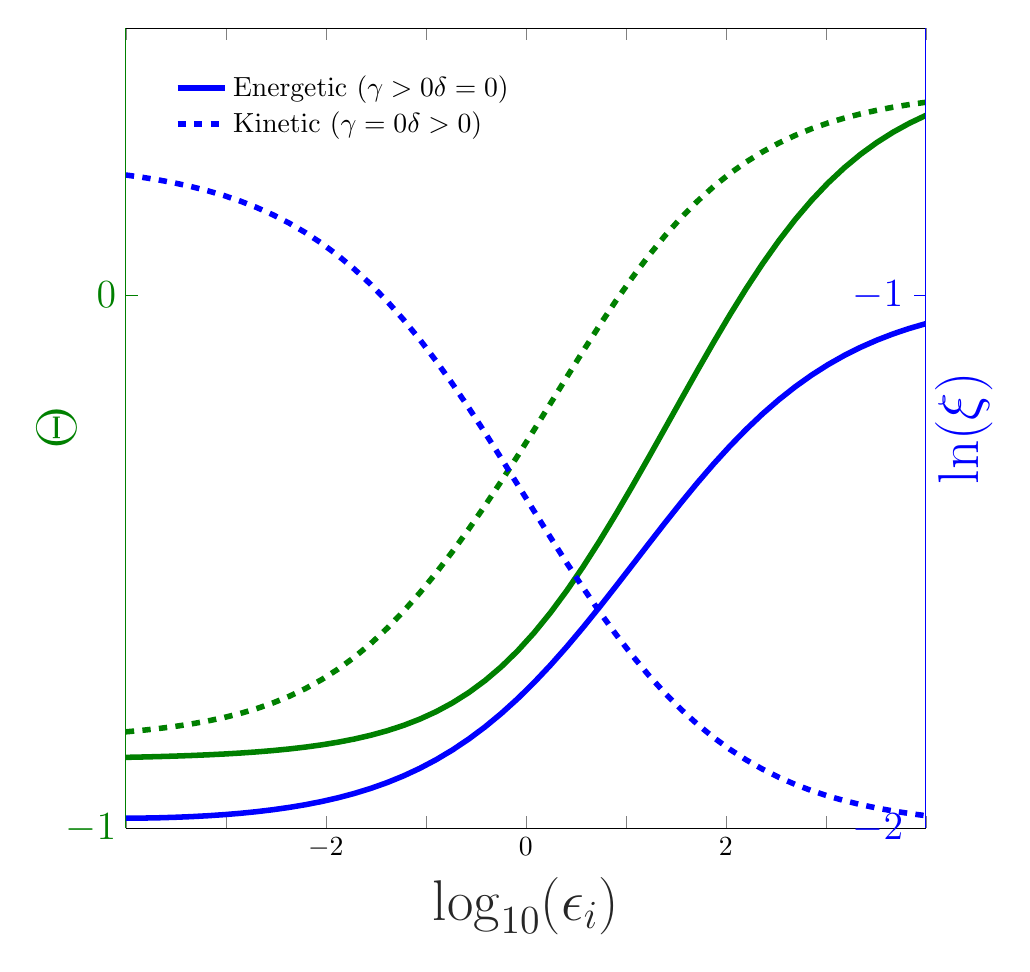
\begin{tikzpicture}

\begin{axis}[%
width=4in,
height=4in,
at={(0in,0in)},
scale only axis,
xmin=-4,
xmax=4,
xtick = {-2,0,2},
xlabel style={font=\huge\color{white!15!black}},
xlabel={$\log_{10}(\epsilon_i)$},
separate axis lines,
axis y line*=left,
every outer y axis line/.append style={black!50!green},
every y tick label/.append style={font=\Large\color{black!50!green}},
every y tick/.append style={black!50!green},
ymin=-1,
ymax=0.5,
ytick={-1, 0},
ylabel style={font=\huge\color{black!50!green}, at={(axis description cs:-0.05,0.5)}},
ylabel={$\Theta$},
axis background/.style={fill=none},
yticklabel pos=right,
]
\addplot [color=black!50!green, line width=2.0pt]
  table[row sep=crcr]{%
-4	-0.86712195063823\\
-3.83673469387755	-0.866459706139752\\
-3.6734693877551	-0.865678189906575\\
-3.51020408163265	-0.86475557792563\\
-3.3469387755102	-0.863665936934352\\
-3.18367346938776	-0.862378416090975\\
-3.02040816326531	-0.86085627230916\\
-2.85714285714286	-0.85905569554162\\
-2.69387755102041	-0.856924395411978\\
-2.53061224489796	-0.854399906776275\\
-2.36734693877551	-0.851407570741511\\
-2.20408163265306	-0.847858152256934\\
-2.04081632653061	-0.843645070263551\\
-1.87755102040816	-0.838641248643482\\
-1.71428571428571	-0.832695656115789\\
-1.55102040816327	-0.82562970449693\\
-1.38775510204082	-0.817233833628389\\
-1.22448979591837	-0.80726484286983\\
-1.06122448979592	-0.795444838492099\\
-0.897959183673469	-0.781463031889889\\
-0.73469387755102	-0.764981970340433\\
-0.571428571428571	-0.745649950371574\\
-0.408163265306122	-0.723121091220409\\
-0.244897959183673	-0.697083503684381\\
-0.0816326530612245	-0.667293932145592\\
0.0816326530612245	-0.633614305190569\\
0.244897959183673	-0.596042655351181\\
0.408163265306122	-0.554729524282433\\
0.571428571428571	-0.509973127376225\\
0.73469387755102	-0.462192880959991\\
0.897959183673469	-0.41188943203243\\
1.06122448979592	-0.359605577480526\\
1.22448979591837	-0.305901913003867\\
1.38775510204082	-0.251352791651361\\
1.55102040816327	-0.196556415902121\\
1.71428571428571	-0.142144604926812\\
1.87755102040816	-0.0887779096369525\\
2.04081632653061	-0.0371198277065357\\
2.20408163265306	0.0122053252255192\\
2.36734693877551	0.0586589016979626\\
2.53061224489796	0.101825813127987\\
2.69387755102041	0.141435331724591\\
2.85714285714286	0.177362780569039\\
3.02040816326531	0.209615375532946\\
3.18367346938776	0.238308104188025\\
3.3469387755102	0.263635665558142\\
3.51020408163265	0.285845149784655\\
3.6734693877551	0.305212329132137\\
3.83673469387755	0.322022821711851\\
4	0.336558248592482\\
};

\addplot [color=black!50!green, dashed, line width=2.0pt]
  table[row sep=crcr]{%
-4	-0.819259085237148\\
-3.83673469387755	-0.816436600053761\\
-3.6734693877551	-0.81310206332122\\
-3.51020408163265	-0.809161928752633\\
-3.3469387755102	-0.804505987746505\\
-3.18367346938776	-0.799004925212739\\
-3.02040816326531	-0.792507905034933\\
-2.85714285714286	-0.784840472540855\\
-2.69387755102041	-0.775803233807122\\
-2.53061224489796	-0.765171991637696\\
-2.36734693877551	-0.752700261698691\\
-2.20408163265306	-0.738125293733678\\
-2.04081632653061	-0.721178752485815\\
-1.87755102040816	-0.701602868600687\\
-1.71428571428571	-0.679171912014443\\
-1.55102040816327	-0.653717117997919\\
-1.38775510204082	-0.625150884190199\\
-1.22448979591837	-0.593483931824915\\
-1.06122448979592	-0.55882862046812\\
-0.897959183673469	-0.521384283325877\\
-0.73469387755102	-0.481406751952637\\
-0.571428571428571	-0.439172189239683\\
-0.408163265306122	-0.394950602920698\\
-0.244897959183673	-0.349002589071998\\
-0.0816326530612245	-0.301603045336879\\
0.0816326530612245	-0.253082089354969\\
0.244897959183673	-0.203863611254387\\
0.408163265306122	-0.154481508535011\\
0.571428571428571	-0.105562941118016\\
0.73469387755102	-0.0577816459859097\\
0.897959183673469	-0.0117953265598192\\
1.06122448979592	0.0318152204206433\\
1.22448979591837	0.0725912351830887\\
1.38775510204082	0.110218876033748\\
1.55102040816327	0.144530624770316\\
1.71428571428571	0.175490575663137\\
1.87755102040816	0.203170442256917\\
2.04081632653061	0.227722367752829\\
2.20408163265306	0.2493528598676\\
2.36734693877551	0.268300310592425\\
2.53061224489796	0.284817080744148\\
2.69387755102041	0.299156155212727\\
2.85714285714286	0.311561844577519\\
3.02040816326531	0.322263794881274\\
3.18367346938776	0.331473546483831\\
3.3469387755102	0.339382961805802\\
3.51020408163265	0.346163959821047\\
3.6734693877551	0.351969117749945\\
3.83673469387755	0.3569328105346\\
4	0.361172649961282\\
};

\end{axis}

\begin{axis}[%
width=4in,
height=4in,
at={(0in,0in)},
scale only axis,
xmin=-4,
xmax=4,
xlabel style={font=\huge\color{white!15!black}},
%xlabel={$\log_{10}(\epsilon_i)$},
xticklabels=\empty,
separate axis lines,
axis y line*=right,
every outer y axis line/.append style={blue},
every y tick label/.append style={font=\Large\color{blue}},
every y tick/.append style={blue},
ymin=-2,
ymax=-0.5,
ytick={-2, -1},
ylabel style={font=\huge\color{blue}},
ylabel={$\ln(\xi)$},
axis background/.style={fill=none},
yticklabel pos=right,
legend style={at={(0.05,0.85)}, anchor=south west, legend cell align=left, align=left, fill=none, draw=none},
y tick label style={xshift={-3em},anchor=west},
]

\addplot [color=blue, line width=2.0pt]
  table[row sep=crcr]{%
-4	-1.98123722630083\\
-3.83673469387755	-1.98098507569647\\
-3.6734693877551	-1.98041596099564\\
-3.51020408163265	-1.97951591044775\\
-3.3469387755102	-1.97826293711223\\
-3.18367346938776	-1.97662665915261\\
-3.02040816326531	-1.97456779767177\\
-2.85714285714286	-1.97203756672901\\
-2.69387755102041	-1.96897697802198\\
-2.53061224489796	-1.96531609352077\\
-2.36734693877551	-1.96097327395976\\
-2.20408163265306	-1.95585448992134\\
-2.04081632653061	-1.94985278596987\\
-1.87755102040816	-1.94284801669057\\
-1.71428571428571	-1.93470700572307\\
-1.55102040816327	-1.92528431282414\\
-1.38775510204082	-1.91442382548764\\
-1.22448979591837	-1.90196141423748\\
-1.06122448979592	-1.88772889507563\\
-0.897959183673469	-1.8715595166127\\
-0.73469387755102	-1.85329511960998\\
-0.571428571428571	-1.83279499011033\\
-0.408163265306122	-1.80994623626516\\
-0.244897959183673	-1.78467526595073\\
-0.0816326530612245	-1.75695964644101\\
0.0816326530612245	-1.72683932838268\\
0.244897959183673	-1.69442597385332\\
0.408163265306122	-1.65990901426636\\
0.571428571428571	-1.62355714622354\\
0.73469387755102	-1.58571429409125\\
0.897959183673469	-1.54678962193927\\
1.06122448979592	-1.50724190030877\\
1.22448979591837	-1.46755930666782\\
1.38775510204082	-1.42823641346829\\
1.55102040816327	-1.38975055232747\\
1.71428571428571	-1.35253984096545\\
1.87755102040816	-1.31698489903049\\
2.04081632653061	-1.2833957181928\\
2.20408163265306	-1.25200441256614\\
2.36734693877551	-1.22296380792583\\
2.53061224489796	-1.1963511712314\\
2.69387755102041	-1.17217593096241\\
2.85714285714286	-1.15039003026085\\
3.02040816326531	-1.13089957007333\\
3.18367346938776	-1.11357658162771\\
3.3469387755102	-1.09827004443767\\
3.51020408163265	-1.08481556977907\\
3.6734693877551	-1.07304344923363\\
3.83673469387755	-1.0627849935446\\
4	-1.05387724783603\\
};
\addlegendentry{Energetic ($\gamma>0\delta=0$)}


\addplot [color=blue, dashed, line width=2.0pt]
  table[row sep=crcr]{%
-4	-0.775217342816201\\
-3.83673469387755	-0.779499644886392\\
-3.6734693877551	-0.78446984017953\\
-3.51020408163265	-0.790239539480914\\
-3.3469387755102	-0.796934171227636\\
-3.18367346938776	-0.804693784190871\\
-3.02040816326531	-0.813673461012692\\
-2.85714285714286	-0.824043159570773\\
-2.69387755102041	-0.835986759864976\\
-2.53061224489796	-0.849700059805028\\
-2.36734693877551	-0.865387442263179\\
-2.20408163265306	-0.883256939452262\\
-2.04081632653061	-0.903513463054251\\
-1.87755102040816	-0.926350064312261\\
-1.71428571428571	-0.95193724975618\\
-1.55102040816327	-0.980410610112542\\
-1.38775510204082	-1.01185731352497\\
-1.22448979591837	-1.0463023418734\\
-1.06122448979592	-1.08369566195231\\
-0.897959183673469	-1.12390175522629\\
-0.73469387755102	-1.16669300822434\\
-0.571428571428571	-1.21174832954486\\
-0.408163265306122	-1.25865798046191\\
-0.244897959183673	-1.3069350043196\\
-0.0816326530612245	-1.35603288870117\\
0.0816326530612245	-1.40536831036891\\
0.244897959183673	-1.45434713244375\\
0.408163265306122	-1.50239137167567\\
0.571428571428571	-1.54896471672523\\
0.73469387755102	-1.59359438245302\\
0.897959183673469	-1.63588759111586\\
1.06122448979592	-1.67554168342151\\
1.22448979591837	-1.71234765050332\\
1.38775510204082	-1.74618760738648\\
1.55102040816327	-1.77702728993695\\
1.71428571428571	-1.80490498754057\\
1.87755102040816	-1.82991841332557\\
2.04081632653061	-1.85221089909396\\
2.20408163265306	-1.8719580480963\\
2.36734693877551	-1.88935565798198\\
2.53061224489796	-1.90460940214291\\
2.69387755102041	-1.91792647484832\\
2.85714285714286	-1.92950918754672\\
3.02040816326531	-1.93955035603465\\
3.18367346938776	-1.94823023414304\\
3.3469387755102	-1.95571471607294\\
3.51020408163265	-1.962154531712\\
3.6734693877551	-1.96768518364264\\
3.83673469387755	-1.97242741029798\\
4	-1.97648799909347\\
};
\addlegendentry{Kinetic ($\gamma=0\delta>0$)}


\end{axis}
\end{tikzpicture}%
}} 
\caption{Orthogonality in the Hopfield-Ninio scheme.  (a) Reaction diagram of the scheme.  Note that in the energetic regime, $k_W$ and $l_W$ will differ from $k_R$ and $l_R$ by a factor $e^{\gamma}$.  In the kinetic regime, $k_R$ and $k^{\prime}_R$ increase by a factor $e^{\delta}$ and $l_W$ and $l^{\prime}_W$ increase by a factor $e^{\delta_p}$ \cite{Rao2015}.  (b) Orthogonality bounds minimum error rate in the energetic regime  ($\gamma=1, \delta=0$). The log of the error rate $(\log(\xi))$ as a function of the orthogonality ($\Theta$) is plotted for simulated data (parameter selection in Methods).   Heatmap coloration represents relative dissipation $\Delta S_i$ \cite{Schnakenberg1976} (hotter is higher dissipation); note that at a given orthogonality level, the error rate decreases as dissipation goes up (more red).  (c) In the energetic  regime, minimum error (red line, $\xi = e^{-2\gamma}$) is achieved by simultaneously minimizing orthogonality ($\Theta$, green) and maximizing dissipation (black).  Excess dissipation drives orthogonality upwards, asymptoting with error equal to the binding energy difference ($\xi = e^{-\gamma}).$   (d) Orthogonality as a function of drive.  In the energetic regime (solid curves), error rate ($\xi$) is minimized in the limit of low orthogonality ($\Theta$). In the kinetic regime, (dashed curves), error rate is minimized in the limit of high orthogonality. \label{fig:hopfield}}
\end{figure*}
